%\documentclass[3p,twocolumn]{elsarticle}
%\documentclass[3p,twocolumn]{svmult}

\documentclass[graybox]{svmult}

\usepackage{color}
\usepackage{graphicx}
\usepackage{url}


%\usepackage[colorlinks=false]{hyperref}

\usepackage{float}
\usepackage{listings}   
\usepackage[small,it]{caption}
\usepackage{ifpdf}    
\usepackage{pdfsync}
\usepackage{fancyvrb}
\usepackage{hyperref}
\usepackage{xspace}
\usepackage{wrapfig}

\usepackage{mathptmx}       % selects Times Roman as basic font
\usepackage{helvet}         % selects Helvetica as sans-serif font
\usepackage{courier}        % selects Courier as typewriter font
\usepackage{type1cm}        % activate if the above 3 fonts are
                            % not available on your system
%
\usepackage{makeidx}         % allows index generation
\usepackage{multicol}        % used for the two-column index
\usepackage[bottom]{footmisc}% places footnotes at page bottom

% see the list of further useful packages
% in the Reference Guide

\makeindex             % used for the subject index
                       % please use the style svind.ist with
                       % your makeindex program

\setlength\parskip{-0.015em}
\setlength\parsep{-0.15em}

\newenvironment{shortlist}{
	\vspace*{-0.85em}
  \begin{itemize}
 \setlength{\itemsep}{-0.3em}
}{
  \end{itemize}
	\vspace*{-0.6em}
}

\DefineShortVerb{\|}
\DefineVerbatimEnvironment{mycode}{Verbatim}
{
  label=Code Example,
  fontsize=\scriptsize,
  frame=single,
% framerule=1pt,
  framesep=0.25em,
  numbers=right,  %numbers=right,
  numbersep=0.5pt,
  gobble=0,
  numberblanklines=false
}
\begin{document}

\title{Application-Level Interoperability Across Grids and Clouds}

\author{Shantenu Jha, Andre Luckow, Andre Merzky, Miklos Erdely, Saurabh Sehgal}

% \small{\emph{$^{1}$Center for Computation \& Technology, Louisiana State University, USA}}\\
%   \small{\emph{$^{2}$Department of Computer Science, Louisiana State University, USA}}\\
%   \small{\emph{$^{3}$Department of Computer Science \& Systems
%       Technology, University of
%       Pannonia, Veszprem, Hungary}}\\
%   \small{\emph{$^{4}$Computer \& Automation Research Institute of the
%       Hungarian Academy of
%       Sciences}}\\
%   \small{\emph{$^{*}$Contact Author \texttt{sjha@cct.lsu.edu}}}
%   \upp\upp\upp\upp\upp }

\institute{Shantenu Jha \at Louisiana State University, Baton Rouge,
  USA 70803 \email{sjha@cct.lsu.edu} \and Andre Luckow \at Louisiana
  Statue University, Baton Rouge, USA 70803
  \email{aluckow@cct.lsu.edu} \and Andre Merzky \at Louisiana State
  University, Baton Rouge, USA 70803 \email{andre@merzky.net} \and
  Miklos Erdely \at University of Pannonia, Veszprem, Hungary
  \email{erdelyim@gmail.com}}


\newif\ifdraft
\drafttrue
\ifdraft
 \newcommand{\amnote}[1]{     {\textcolor{magenta} { ***AM: #1 }}}
 \newcommand{\jhanote}[1]{    {\textcolor{red}     { ***SJ: #1 }}}
 \newcommand{\miklosnote}[1]{ {\textcolor{blue}    { ***ME: #1 }}}
 \newcommand{\ssnote}[1]{     {\textcolor{blue}    { ***SS: #1 }}}
 \newcommand{\alnote}[1]{     {\textcolor{blue}    { ***AL: #1 }}}
\else
 \newcommand{\amnote}[1]{}
 \newcommand{\jhanote}[1]{}
 \newcommand{\miklosnote}[1]{}
 \newcommand{\ssnote}[1]{}
  \newcommand{\alnote}[1]{}
\fi

\newcommand{\sagamapreduce}{SAGA-MapReduce\xspace}
\newcommand{\smr}{\sagamapreduce}
\newcommand{\mr}{MapReduce\xspace}
\newcommand{\tc}{$T_c$\xspace}
\newcommand{\wc}{wordcount\xspace}
\newcommand{\Wc}{Wordcount\xspace}

\newcommand{\dn}{\vspace*{0.33em}}
\newcommand{\dnn}{\vspace*{0.66em}}
\newcommand{\dnnn}{\vspace*{1em}}
\newcommand{\uppp}{\vspace*{-1em}}
\newcommand{\upp}{\vspace*{-0.66em}}
\newcommand{\up}{\vspace*{-0.33em}}
\newcommand{\shift}{\hspace*{1.00em}}

\newcommand{\T}[1]{\texttt{#1}}
% \newcommand{\I}[1]{\textit{#1}}
\newcommand{\B}[1]{\textbf{#1}}
\newcommand{\F}[1]{\B{[FIXME: #1]}}
\newcommand{\TODO}[1]{\textcolor{red}{\B{TODO: #1}}}

\newcommand{\ssh}[1]{\T{ssh}\xspace}
\newcommand{\scp}[1]{\T{scp}\xspace}
\newcommand{\sshfs}[1]{\T{sshfs}\xspace}
 

\maketitle
%\begin{abstract}

\abstract{Application-level interoperability is defined as the ability of an
  application to utilise multiple distributed heterogenous resources.
  Such interoperability is becoming increasingly important with
  increasing volumes of data, multiple sources of data as well as
  resource types.  The primary aim of this Chapter is to understand
  different ways in which application-level interoperability can be
  provided across distributed infrastructure. We achieve this by, (i)
  using the canonical \wc application, based on an enhanced version of
  \mr that scales-out across clusters, clouds and HPC resources, (ii)
  establishing how SAGA enables the execution of \wc application using
  \mr and other programming models such as Sphere concurrently, and
  (iii) demonstrating the scale-out of ensemble-based bio-molecular
  simulations across multiple resources.  We We show user-level
  control of the relative placement of compute and data and also
  provide simple performance measures and analysis of \sagamapreduce
  when using multiple, different, heterogeneous infrastructures
  concurrently for the same problem instance. Finally, we discuss
  Azure and some of the system-level abstractions that it provides and
  show how it is a used to support ensemble-based bio-molecular
  simulations.}

%\end{abstract}
%\maketitle

\section{Introduction}\label{sec:intro}


\jhanote{The aim of this chapter is to convert the interop paper into
  a book chapter, by adding some context from an earlier book chapter,
  by adding some Azure work (cut and paste from proposal) and
  hopefully by getting saurabh + miklos to do tests/performance
  numbers on FutureGrid.  at least the figure comparing SAGA-Mapredcue
  and SAGA-Sphere should be extended to a couple of more platforms}

There are numerous scientific applications that either currently
utilize, or need to utilize data and resources distributed over vast
heterogeneous infrastructures and networks with varying speeds and
characteristics. Many distributed frameworks are however, designed
with infrastructures; dependence and tight-coupling to specific
resource types and technology, in a heterogeneous distributed
environment is not an optimal design choice.
In order to leverage the flexibility of distributed systems and to
gain maximum runtime performance, applications must shed their
dependence on single infrastructure for all of their computational and
data processing needs. For example, the Sector/Sphere data cloud is
exclusively designed to support data-intensive computing on high speed
networks, while other distributed file systems like GFS/HDFS assume
limited bandwidth among infrastructure nodes ~\cite{GFS, HDFS}. Thus,
for applications to efficiently utilize heterogeneous environments,
abstractions must be developed for the efficient utilization of and
orchestration across such distinct distributed infrastructure. 

% We define the ability of an application to utilise multiple
% distributed heterogenous resources as application-level interop
% \jhanote{Introduce IDEAS and explain how ``I'' is the basis upon
%   which DEAS are built/predicated}

In addition to issues of performance and scale addressed in the
previous paragraph, the transition of existing distributed programming
models and applications to emerging and novel distributed
infrastructure must be as seamless and as non-disruptive as
possible.  A fundamental question at the heart of all these 
considerations is the question of how scientific applications can be
developed so as to utilize as broad a range of distributed systems as
possible, without vendor lock-in, yet with the flexibility and
performance that scientific applications demand.

% Additionally, there are infrastructure specific features --
% technical and policy, that might influence the design of PM and
% PS. For example, EC2 -- the archetypical cloud system, has a
% well-defined cost model for data transfer across {\it its}
% network. Hence, any PM for clouds should be cognizant of the
% requirement to programmatically control the placement of compute and
% data relative to each other -- both statically (pre-run time) and
% dynamically (at run-time).  In general, for most cloud applications
% the same computational task can be priced very differently for
% possibly the same performance; conversely, the same computational
% task can have very different performance for the same price.

We define Application Level Interoperability (\I{ALI}) as a feature
that arises, when other than say compiling, there
are no further changes required of the application to utilize a new
platform.  If service-level interoperability can be considered as weak
interoperability, ALI can be considered to be {\it strong}
interoperability.  
The complexity of providing ALI varies and depends upon the
application under consideration.  For example, it is somewhat easier
for simple ``distribution unaware'' applications to utilize multiple
heterogeneous distributed environments, than for applications where
multiple distinct and possibly distributed components need to
coordinate and communicate.  

% A pre-requisite for ALI is infrastructure independent programming. 

\paragraph{The Case for Application-level Interoperability}

ALI is not only of theoretical interest. There exist many application
which involve large volumes of data on distributed heterogeneous
resources. For examples, the Earth-Science Grid involves peta to
exa-bytes of data, and one thus cannot move all data (given
current transfer capabilities), nor compute at a centralized location.
Thus there is an imperative to operate on the data {\it in situ},
which in turn involves computation across heterogeneous distributed
platforms as part of the same application.
 
In addition, there exist a wide range of applications that have
decomposable but heterogeneous computational tasks. It is conceivable,
that some of these tasks are better suited for traditional grids,
whilst some are better placed in cloud environments.  The LEAD
application, as part of the VGrADS project provides a prominent
example\footnote{\url{http://vgrads.rice.edu/presentations/VGrADS_overview_SC08pdf.pdf}}.
Due to different data-compute affinity requirement amongst the tasks,
some workers might be better placed on a cloud~\cite{jha_ccpe09},
whilst some may optimally be located on regular grids. Complex
dependencies and inter-relationships between sub-tasks make this often
difficult to determine before run-time. 

Last, but not least, in the rapidly evolving world of clouds, there is
as of yet little business motivation for cloud providers to define,
implement and support new/standard interfaces. Consequently, there is
a case to be made that by providing ALI, such barriers can be overcome
and cross-cloud applications can be easily achieved.
 
Ideally, an application can utilize any PM, and any PM should be
executable on any underlying infrastructure. However, an application
maybe better suited to a specific PM; similarly a specific PM maybe
optimised for a specific infrastructure. But where this is not
necessarily the case, or more importantly, where/when different
application or PM can utilise ``non-native'' infrastructure, mix and
match across the layers of application, PM and infrastructure should
be supported.  Currently, many programming models and abstractions are
tied to a specific back-end infrastructure.  For example, Google's
MapReduce, which is tied to Google's file system, or
Sphere\cite{sectorsphere09} which is linked to the Sector file
system. Thus there is a need to investigate interoperability of
different programming models for the same application on different
systems.


% It is unclear what kind of programming models (PM) and
% programming systems (PS) will emerge for clouds; this will depend,
% amongst other things, on the kinds of applications that will come
% forward to try to utilize clouds and system-level interfaces that are
% exposed by cloud providers.  However, 
% It is important for effective
% scientific application development on clouds that any PM is not
% constrained to a specific infrastructure.  

% \jhanote{Place somewhere appropriate} Counterexamples are Google's
% MapReduce, which is tied to Google's file system, or
% Sphere\cite{sectorsphere09} which is linked to the Sector file system.
 
% An application may be better suited to execution using different
% programming models on different systems.  

%It is also the aim of our studies to 

% Finally, effort directed towards ALI on clouds/grids in addition to
% satisfying basic curiosity of ``if and how to interoperate'', might
% also possibly provide different insight into the programming
% challenges and requirements.  

% Additionally, with different clouds providers, fronting different
% Economic Models of computing, it is important to be able to utilize the
% ``right resource'', in the right way. We briefly discussed how moving
% prodigious amounts of data across cloud networks, as opposed to moving
% the compute unit, could be expensive.  As current programming models
% don't provide explicit support or control for
% affinity~\cite{jha_ccpe09}, and in the absence of autonomic performance
% models, the end-user is left with performance management, and with the
% responsibility of explicitly determining which resource is optimal.
% Clearly interoperability between different flavors of clouds, and
% clouds and grids is an important pre-requisite.  

% which is an application with multiple homogeneous workers (although
% the data-load per worker can vary) however, it is easy to conceive of
% an application where workers (tasks) can be heterogeneous, i.e., each
% worker is different and may have different data-compute ratios. 

In our effort to understand these issues, to establish and investigate
ALI, we will work with MapReduce and an application based on \mr --
the canonical \wc application.  We use SAGA --- “Simple API for Grid
Applications'' (see Sec.~\ref{sec:saga}) as the programing system.  In
Ref.~\cite{saga_ccgrid09}, for example, we implemented a simple \mr
based \wc application using SAGA.  We demonstrated that the SAGA-based
implementation is infrastructure independent, whilst still providing
control over deployment, distribution and run-time decomposition.
We demonstrated that \sagamapreduce is interoperable on traditional
(grids) and emerging (clouds) distributed infrastructure
\I{concurrently and cooperatively towards a solution of the same
  problem instance}.  Our approach was to % take \sagamapreduce and to
use the \I{same} %instance of \sagamapreduce to solve the same
instance of the {\wc}ing problem, by using different worker
distributions over clouds and grid systems.

A primary focus of this chapter is to build upon and use SAGA-based
MapReduce as an exemplar to discuss multiple levels and types of
interoperability that can exist between grids and clouds. We will
also, show that our approach to ALI helps break the coupling between
programming models and infrastructure on the one hand, whilst
providing empirically-driven insight about the performance of an
application with different programming models.

% and thereby also test for interoperability between different flavors
% of clouds as well as between clouds and grids.

% this involved the concurrent execution of simple,
% embarrassingly-parallel data-analysis tasks.

This paper is structured as follows: Section~\ref{sec:saga} gives a
short overview over those SAGA extensions which enable specifically
the ALI work discussed in this paper.  Section~\ref{sec:mr} describes
our \smr implementation.  Section~\ref{sec:interop} discusses the
different levels of ALI we are demonstrating with this paper, with
more details on the experiments in Section~\ref{sec:exp}.  We change
the focus to a more traditional compute-intensive applications in
Section 6; although very commonly used and needed, it still remains a
challenge to effectively utilize multiple resources for the effective
solution of ensemble-based simulations. This provides the motivation
for our work in \S6. In \S7, we discuss Azure in the context of
ensemble-based bio-molecular simulations. Section~\ref{sec:discuss}
concludes the paper with a discussion of the results.

% Thanks to the ease of
% developing SAGA “Adaptors”, developers can provide SAGA the interfaces
% to interact with widely different infrastructures simultaneously
% throughout the execution of a single application.

% It is worth mentioning that most
% data-intensive scientific applications fall into this category e.g.,
% high-energy and LIGO data-analysis.  


\section{SAGA}
\label{sec:saga}

The SAGA~\cite{saga-core, Kaiser:2006qp} programming system provides a
high level API that forms a simple, standard and uniform interface for
the most commonly required distributed functionality.  SAGA can be
used to program distributed applications~\cite{saga_escience07,
saga_tg08} or tool-kits to manage distributed
applications~\cite{Luckow:2008xy}, as well as implement abstractions
that support commonly occurring programming, access and usage
patterns.

\begin{figure}[t]
 \centering
 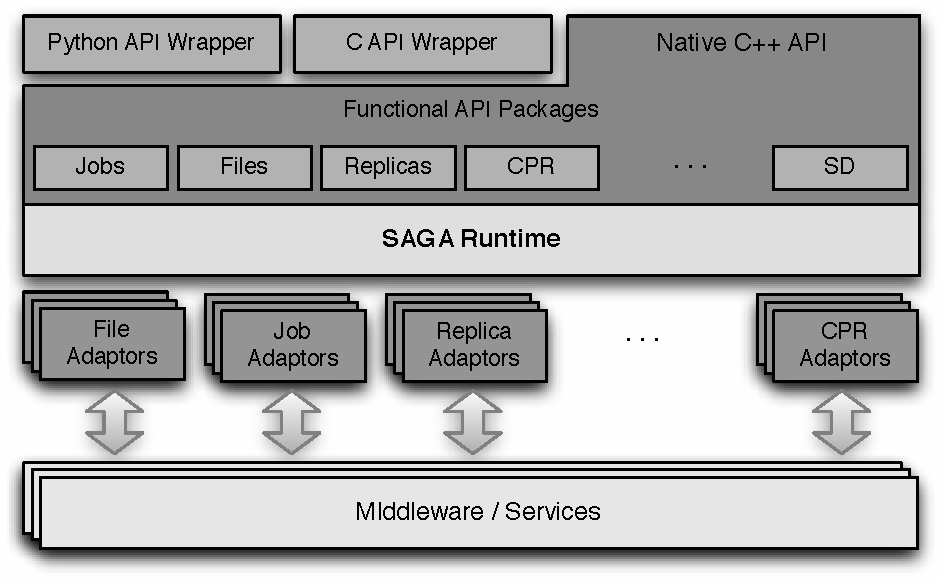
\includegraphics[width=0.8\textwidth]{figures/saga-figure02-gray.pdf}
 \caption{The SAGA runtime engine dynamically dispatches high level
          API calls to a variety of middlewares.}
 \label{fig:saga}
 \alnote{Do we have a scalable vector graphic version?}
\end{figure}

Fig.~\ref{fig:saga} provides an overview of the SAGA programming
system's architecture.  The SAGA API covers job submission, file
access and transfer, as well as logical file management.  Additionally
there is support for Checkpoint and Recovery (CPR), Service Discovery
(SD), and other areas.  The API is implemented in C++ and Java, with
Python supported as a wrapper. \I{saga\_core} is the main library,
which provides dynamic support for run-time environment decision
making through loading relevant adaptors. We will not discuss SAGA
internals here; details can be found elsewhere~\cite{saga_url,Kaiser:2006qp}.


\subsection{Interfacing SAGA to Grids and Clouds}

SAGA was originally developed primarily for compute-intensive grids.
Ref~\cite{saga_ccgrid09} demonstrated that in spite of its original
design constraints, SAGA can be used to develop data-intensive
applications in diverse distributed environments, including clouds.
This is in part due to the fact that, at least on application level,
much of the ``distributed functionality'' required for data-intensive
applications remains the same.  How the respective functionality for
grid systems and for EC2 based cloud environments is provided in SAGA
is also documented in~\cite{saga_ccgrid09}.  Based on those
experiences, we added another backend to the set, which allows to
extend the range of backend architectures available to SAGA-C++ to
Sector-Sphere~\cite{sectorsphere09}.

% Several illustrative and popular programming abstractions such as
% Map-Reduce and All-Pairs \cite{allpairs} have been successfully
% implemented with SAGA, thus showcasing its utility n as a flexible
% framework to scale-out data-intensive computations on different
% flavors of grids and clouds, and attain a high level of
% interoperability at the application level.


\subsection{Sector-Sphere Adaptors: Design and Implementation}

Sector and Sphere is a cloud framework specifically designed for
writing applications able to utilize the stream processing paradigm.
Sector is a distributed file system that manages data across physical
compute nodes at the file level, and provides the infrastructure to
manipulate data in the cloud.  Sphere, on the other hand, provides the
framework to utilize the stream processing paradigm for processing the
data residing on Sector.  The Sphere system is composed of Sphere
Processing Engines (SPEs) running on the same physical nodes as the
Sector file system.

Applications that utilize the stream processing paradigm define a
single common function (aka kernel) that is applied to segments of a
given data set.  When the application invokes Sphere to process data
on Sector, the Sphere system retrieves the stream of data, segments
the data and assigns chunks of these segments to the available SPEs
for processing.

Sphere allows the user to encode the kernel function in a dynamically
linked library written against the Sphere APIs.  The SPEs apply this
user defined function to its assigned segments and write the
processing results back to files in Sector.  This stream of output
files can be retrieved by the user from Sector, after the processing
is complete. 

% \ssnote{Maybe add a different section here}
% \ssnote{Add another section here for experiments, or maybe later after
% MapReduce description} 

\paragraph{SAGA Adaptor Overhead} \label{ssec:overhead}

We execute a simple experiment to measure the overhead introduced by
submitting Sphere jobs and Sector file operations through SAGA.  The
used sample Sphere kernel function accepts a buffer of text and
utilizes the Sphere framework to hash words into Sphere buckets, using
the first letter as the key. One Gigabyte of text data was uploaded to
the Sector file system for this test.  Furthermore, traces were
implemented in the adaptors to measure the exact time spent in SAGA
processing and translation before the raw Sphere APIs were called.  As
seen in Table ~\ref{tab:sphere_overhead}, the SAGA overhead is, if compared
to the overall execution time of the application, negligible.
This makes SAGA an excellent platform to compare Sphere with other distinct
programming models.

\begin{table}
\centering
  \footnotesize
  \begin{tabular}{cccc}
    \hline
    & Vanilla Sphere &  SAGA-Sphere & Adaptor \\
    &                &              & overhead \\
    \hline
    { {\bf Mean}} & 3.2    & 4.1    & 0.43  \\
    \hline 
    { {\bf Stdev}} & 0.5    & 1.2    & 0.07   \\
    \hline \hline
  \end{tabular}
  \caption{Adaptor overhead measurements from processing 8GBs of data with 8
  SPEs running the \wc application on 8 physical nodes on Poseidon (a
  LONI cluster).  All times are in minutes, aggregated from 10 runs.
  \label{tab:sphere_overhead}}
\end{table}

Thanks to the low overhead of developing SAGA adaptors, we were able
to implement the Sector file adaptor, and the Sphere job adaptor for
applications to utilize the stream processing paradigm through SAGA.
\miklosnote{Andre/Saurabh: could you please give API examples for file/job
support for Sector/Sphere in SAGA?}
%\F{Figure} and \F{Figure} give simple examples of how SAGA APIs
%can be used to manipulate data in the Sector systems, and how jobs can
%be submitted to the Sphere system to process this data.
The enhancement of \sagamapreduce, along with the implementation of the
Sector/Sphere adaptors naturally gives us the opportunity to compare
and study these two distinct programming models.


\section{SAGA-based MapReduce}
\label{sec:mr}

 Given its relevance~\cite{saga_ccgrid09}, we choose the \smr
 implementation to compare both, different backend systems (grids,
 clouds, and clusters) and different programming models (master/slave,
 Sector-Sphere streams).  A simple \wc application on top of
 \smr has been used as a close-to-reality test case, and is
 described in Sec.~\ref{ssec:app}.

% After \sagamapreduce we have also developed real scientific
% applications using SAGA based implementations of patterns for
% data-intensive computing: multiple sequence alignment can be
% orchestrated using the SAGA-All-pairs implementation, and genome
% searching can be implemented using SAGA-MapReduce (see
% Ref.~\cite{saga_ccgrid09}).
% \upp

\subsection{\sagamapreduce Implementation}\label{ssec:app}

Our implementation of \sagamapreduce interleaves the core \mr logic
with explicit instructions on where processes are to be scheduled.
The advantage of this approach is that our implementation is no longer
bound to run on a system providing the appropriate semantics
originally required by MapReduce, and is portable to a broader range
of generic systems as well.  The drawback is that it is more
complicated to extract performance, as some system level semantics has
to be recreated in application space (i.e., on SAGA or \smr) level.
% -- for there is a need to add system
% semantic capabilities at some level, and it is inherently slower --
% as it is difficult to reproduce system-specific optimizations to
% work generically.
The fact that the implementation is single-threaded proved to be the
primary current performance inhibitor.  However, none of these
complexities are exposed to the end-user, as they remain hidden within
the framework. 

% Also many of the complexities are due to the early-stages of SAGA
% and incomplete implementation of features, and not a fundamental
% limitation of the design or concept of the interface or programming
% models that it supports.  Future SAGA API packages will allow to
% alleviate some of these issues.

% The overall architecture of the SAGA-MapReduce implementation is
% shown in Fig.~\ref{saga-mapreduce_controlflow}. 
\smr exposes a simple interface which provides the complete
functionality needed by any MapReduce algorithm, while hiding the more
complex functionality, such as chunking of the input, sorting the
intermediate results, launching and coordinating the workers, etc. --
these are generically implemented by the framework.  The application
consists of two independent processes, a master and worker processes.
The master process is responsible for:

\begin{itemize}

 \item launching all workers for the map and reduce steps, as
 described in a configuration file provided by the user; and

 \item coordinating the workers, chunking of the data, assigning the
 input data to the workers of the map step, handling the intermediate
 data files produced by the map step, passing the location of the
 sorted output files to the workers of the reduce step.  

% \item re-launching single worker instances in case of failures, thus
% providing fail safety.
% \miklosnote{fail safety since it's not actually present.

\end{itemize}

When launching a job, the master is the executable run by the client
itself which means the resource from which the client program is run
determines from where the master will be available.  A MapReduce job
is specified by a JobDescription object in which the user sets the
Mapper and Reducer classes, input and output paths and formats.  The
used InputFormat creates the logical partitions of the input data for
the master which information is then sent to idle workers.  A
Raw\-Record\-Reader implementation is responsible for interpreting an
InputChunk and providing a record iterator for the Mapper. It is
possible to support any kind of data source for which a record
oriented view makes sense by writing a custom Raw\-Record\-Reader.
The output from the Mapper is further processed by the Partitioner
which assigns emitted key/value pairs from the Mapper to reducers.
Finally, a Raw\-Record\-Writer writes output data to files.  Custom
Raw\-Record\-Writer and Partitioner classes can be also implemented to
suit an application's needs.  \miklosnote{Andre/Shantenu: Please check
coherence of the above paragraph.}

The master process is readily available to the user and needs no
modification for different map and reduce functions to execute.  The
worker processes get assigned work either from the map or the reduce
step. The functionality for the different steps have to be provided by
the user, which means the user has to write two C++ functions
implementing the respective MapReduce kernels.

Both the master and the worker processes use the SAGA-API as an
abstract interface to the used infrastructure, making the application
portable between different architectures and systems.  The worker
processes are launched using the SAGA job package, allowing the jobs
to launch either locally, on Globus/GRAM backends, on EC2 instances, through SSH
or on a Condor pool. The communication between the master and workers
is ensured by using the SAGA advert package, abstracting an
information database in a platform independent way, and the SAGA stream
package, abstracting streaming data access between network endpoints.
The master creates logical partitions of the data (referred to as chunking,
analogous to Google's MapReduce), so the data-set does not have to be split
and distributed manually.  The input data can be located on any file system
supported by SAGA, such as the local file system or a distributed file system
like HDFS or KFS \cite{KFS}.


\subsection{Enhancing SAGA-based Map-Reduce Performance}

The performance enhancements to the \sagamapreduce implementation as
discussed in~\cite{saga_ccgrid09} are based on two important changes:
(i) rearranging the shuffle phase, and (ii) using a serialized binary
format instead of plain text for intermediate data storage (also
available as an input and output format).  The first change means
that, instead of having the master merge and then sort the
intermediate data by key before entering the reduce phase, the workers
buffer key/value pairs from the map phase and store them in sorted
order on disk, doing an in-memory sort before writing. Also, since
intermediate key/value pairs from a map worker are already sorted, the
reduce workers need to only merge these pairs coming from different
map workers while applying the user-defined reduce function to the
merged intermediate key and value list.  The second enhancement
applies to the storage of the intermediate key/value pairs in a
so-called \emph{sequence file format}. This file format allows storing
of serialized key/value objects which can be read and merged much
faster in the reduce phase than text data, as there is no need for
costly parsing.  We used the Google Protocol Buffers library for
implementing serialization~\cite{protobuf}.  The processing of input
and output key/value pairs is further enhanced by minimizing
unnecessary memory I/O operations using a zero-copy scheme.

\jhanote{(A) Why do we think these are the most important performance
  enhancements that should be attempted? Or was/is it a case of -- we
  can, therefore we do? (B) Can the performance improvement that arise
  from (i) and (ii) be quantified separately?  (C) What other
  improvements can be and should be implemented?}
  

\subsection{\sagamapreduce Set-Up}

As with any application which concurrently spans multiple diverse
resources or infrastructures, the coordination between the different
application components becomes challenging.  The \smr implementation
uses the SAGA advert API for that task, and can thus limit the a-priori
information needed for bootstrapping the application: the compute
clients (workers) require (i) the contact address of the used advert
service instance, and (ii) a unique worker ID to register with in that
advert service, so that the master can start to assign work items.
Both information are provided by the master via command line
parameters to the worker, at startup time.

The master application requires the following additional information:
(i) a set of resources where the workers can execute, (ii) the
location of the input data, (iii) the target location for the output
data, and (iv) the contact point for the advert service for
coordination and communication.  

In a typical configuration, for example, three worker instances could
be started; the first could be started via GRAM and PBS on
qb.teragrid.org, the second on a pre-instantiated EC2 image
(instance-id \T{i-760c8c1f}), and the third on a dynamically deployed
EC2 instance (no instance id given).  Note that the startup times for
the individual workers may vary over several orders of magnitudes,
depending on the PBS queue waiting time and VM startup time.  The
MapReduce master will start to utilize workers as soon as they are
able to register themselves, so will not wait until all workers are
available.  That mechanism both minimizes time-to-solution, and
maximizes resilience against worker loss.
%
% The scheme \T{any} acts here as a placeholder for SAGA, so that the
% SAGA engine can choose an appropriate adaptor.  The master would
% access the file via the default local file adaptor.  The globus
% clients may use either the GridFTP or SSH adaptor for remote file
% success (but in our experimental setup would also succeed using the
% local file adaptor, as the Lustre FS is mounted on the cluster
% nodes), and the EC2 workers would use the ssh file adaptor for
% remote access.  Thus, the use of the placeholder scheme frees us
% from specifying and maintaining a concise list of remote data access
% mechanisms per worker.  Also, it facilitates additional resilience
% against service errors and changing configurations, as it leaves it
% up to the SAGA engine's adaptor selection mechanism to find a
% suitable access mechanism at runtime.  A parameter not shown in the
% above configuration example 
%
A simple parameter controls the number of workers created on each
compute node; as we will see by varying this parameter, the chances
are good that compute and communication times can be interleaved, and
that the overall system utilization can increase (especially in the
absence of precise knowledge of the execution system).
 

\section{Application Level Interoperability: Three-levels}
\label{sec:interop}

The motivation of ALI across multiple, heterogeneous and distributed
resources follows from large-scale scientific applications, such as
the Earth Science Grid and LEAD. However for simplicity of treatment
and to focus on the levels of interoperability we will use a simple,
self-contained application, that has also become the {\it canonical}
\mr application-driver -- \wc.%
%
%\subsection{Interoperability Types}
%
Using the \wc application, we will demonstrate three types of
application level interoperability. We outline them here:

% different levels/types of interoperability.

\subsection{Type I: Application Interoperability via adaptors}
%
% Type I:  Application 
%              |
%           SAGA-MR
%              |
%           Adaptors
%      /     /   \      \
%    ... Clouds  Grids ...
%

As discussed, SAGA provides the ability to load a wide-range of
system-specific adaptors dynamically. Thus a simple form of
interoperability, possibly specific to applications developed using
SAGA, is that an application can use any distributed systems without
changes to the application, thus experiencing cloud-cloud or
grid-cloud interoperability.  We refer to this as Type I
interoperability.

% interoperability quite trivially thanks to the dynamic loading of
% adaptors.  A

Thanks to the relative simplicity of developing SAGA adaptors, SAGA
has been successful interfaced to three cloud systems -- Amazon's EC2,
Eucalyptus~\cite{eucalyptus} (a local installation of Eucalyptus at
LSU) and Nimbus~\cite{nimbus}; and also to a multitude of grid based
environments, including TeraGrid, Loni and NGS.  SAGA based
applications are thus inherently able to utilize this form of ALI.

\subsection{Type II: Application Interoperability using programming
  models} % suited for different infrastructure}
%
% Type II:      Application 
%                    |
%          Instance-1 Instance-2
%            |            |
%         SAGA-Sphere SAGA-MapReduce
%            |            |
%       Sector-Sphere cluster/grids
%

Interoperability at a higher level than adaptors is both possible and
often desirable. An application can be considered interoperable if it
is able to switch between backend specific programming models.  We
will discuss an example where the \wc application is implemented so
that it can utilize either a Sector-Sphere framework via SAGA for the
OCC backend, or the \smr framework for generic grid and cloud
backends.

\subsection{Type III: Application Interoperability using different
  programming models for concurrent execution}
%
% Type III:   Application
%                 |
%     SAGA-Sphere / SAGA-MapReduce
%                 |
%   Sector-Sphere / cluster / grids / clouds
%

At another level, an application can also be considered interoperable
when it executes multiple programming models \I{concurrently} over
diverse backends.  We demonstrate that a \wc application uses both
Sector-Sphere and \smr when spanning  multiple backends.  The
challenges of having different parts of an application execute
concurrently using different programming models is conceptually
different to loading different adaptors concurrently. Thus we describe
this as a separate type of interoperability.

\subsection{Experimental Setup}
\alnote{WE should consider to move this subsection to ~\ref{sec:exp}}
Simulations were performed on shared TeraGrid-LONI (Louisiana Optical
Network Initiative)~\cite{loni-url} resources running Globus and ssh;
on GumboGrid, a small cluster at LSU running Eucalyptus; on Amazon's
EC2; on a bare 50 node cluster of the Hungarian Academy of Sciences;
and on the OCC testbed~\cite{occ_testbed} running Sector-Sphere.  Jobs
are started via the respectively available middlewares, via SAGA's job
API.  Data exchange is either performed via streams, or via SAGA's
file transfer API which can dynamically switch between the various
available protocols.

For cloud environments, we support the runtime configuration of VM
instances by staging a preparation script to the VM after its
creation, and executing it with root permissions.  In particular for
apt-get Linux distribution, the post-instantiation software deployment
is actually fairly painless, but naturally adds a significant amount
of time to the overall VM startup (which encourages the use of
preconfigured images).

For experiments in this paper, we prepared custom VM images with
pre-installed prerequisites.  We utilize preparation scripts solely
for some fine tuning of parameters: for example, to deploy custom
saga.ini files, or to ensure the finalization of service startups
before application deployment.

Deploying \sagamapreduce framework and the \wc application on
different grids, clouds or clusters requires adapting the configuration
to the specific environment.  For example, when running \sagamapreduce
on EC2, the master process resides on one VM, while workers reside on
different VMs.  Depending on the available adaptors, Master and Worker
can either perform local I/O on a global/distributed file system, or
remote I/O on a remote, non-shared file system.

It must be noted that we utilized different \smr versions for the
described experiments: the work described in this paper spans more
than 18 months, and the \smr implementation has simply evolved over
time.  As our primary goal is to demonstrate interoperability, and not
to document maximal performance, we consider those results valid
nonetheless.

\section{Interoperability Experiments: \Wc}
\label{sec:exp}


We use our own implementations of the well known \wc application for
our experiments.  \Wc has a well understood runtime and scaling
behaviour, and thus serves us well for focusing the tests on the used
frameworks and middlewares.

The \mr based \wc implementation is described in~\cite{saga_ccgrid09}.
For the Sector-Sphere version of \wc we implemented two kernel
functions. The first one is responsible for hashing the
words in the data set into different "buckets", depending on
the word's starting letter.  The standard C++ collate hashing function
was used for this purpose.  The second kernel function reads each hash
bucket, sorts the words in memory and outputs the final count of
the words in the data set.  For example, a file containing the words
\T{('bread' 'bee' 'bee' 'honey')} would be hashed into buckets as
\T{('bread' 'bee' 'bee')} and \T{('honey')}.  The second kernel
function would read these intermediate bucket files, sort the words,
and produce the result \T{(.bread 1., .bee 2., .honey
  1.)}.  The Sphere system is responsible for assigning files for
processing, synchronization, and writing output results back to
Sector.

\subsection{Type I ALI: Interoperability via Adaptors}

In an earlier paper (Ref~\cite{saga_ccgrid09}), we performed tests to
demonstrate how \sagamapreduce utilizes different infrastructures and
provides control over task-data placement; this led to insight into
performance on ``vanilla'' grids.  This work extends earlier work and
establishes that \sagamapreduce can provide cloud-cloud
interoperability and cloud-grid interoperability.  We performed the
following experiments:

\begin{enumerate}

 \item We compare the performance of \sagamapreduce when exclusively
 running on a cloud platform to that when on grids. We vary the number
 of workers (1 to 10) and the data-set sizes varying from 10MB to 1GB.

 \item For clouds, we then vary the number of workers per VM, such
 that the ratio is 1:2 and 1:4, respectively.

 \item We then distribute the same number of workers across two
 different clouds - EC2 and Eucalyptus.

 \item Finally, for a single master, we distribute workers across
 grids (QueenBee on the TeraGrid) and clouds (EC2 and Eucalyptus) with
 one job per VM.

\end{enumerate}

It is worth reiterating, that although we have captured concrete
performance figures, it is not the aim of this work to analyze the
data and provide a performance model. In fact it is difficult to
understand performance implications, as a detailed analysis of the
data and understanding the performance will involve the generation of
``system probes'', as there are differences in the specific cloud
system implementation and deployment.  In a nutshell without adjusting
for different system implementations, it is difficult to rigorously
compare performance figures for different configurations on different
machines. At best we can currently derive trends and qualitative
information.  Any further analysis is considered out of scope for this
paper.

It takes SAGA about 45s to instantiate a VM on Eucalyptus and about
200s on average on EC2.  We find that the size of the image (say 5GB
versus 10GB) influences the time to instantiate an image, but is
within image-to-image instantiation time fluctuation.  Once
instantiated, it takes from 1-10s to assign a job to an existing VM on
Eucalyptus, or EC2.  The option to tie the VM lifetime to the
\T{saga::job\_service} object lifetime is a configurable option.  It
is also a matter of simple configuration to vary how many jobs (in
this case workers) are assigned to a single VM:  the default is 1
worker per VM.  The ability to vary this number is important -- as
details of actual VMs can differ as well as useful for our
experiments.


\subsubsection*{Results and Analysis}

The total time-to-solution ($T_s$) of a \sagamapreduce job can be
decomposed as the sum of three primary components -- $t_{pre},
t_{comp}$ and $t_{coord}$.  Here $t_{pre}$ is defined as
pre-processing time, which covers the time to chunk the data into
fixed size data units, to distribute them, and also to spawn the job.
$t_{pre}$ does not include the time required to start VM instances.
$t_{comp}$ is the time to actually compute the map and reduce function
on a given worker, whilst $t_{coord}$ is the time taken to assign the
payload to a worker, update records and to possibly move workers to a
destination resource; in general, $t_{coord}$ scales as the number of
workers increases.

Table~\ref{tab:1a} shows performance measurements for a variety of
worker placement configurations.  The master places the workers on
either clouds or on the TeraGrid (TG). The configurations -- separated
by horizontal lines, are classified as either all workers on the TG or
having all workers on EC2. For the latter, unless otherwise indicated
parenthesis, every worker is assigned to a unique VM. In the final set
of rows, the number in parenthesis indicates the number of VMs used.
Note that the spawning times depends on the number of VMs, even if it
does not include the VM startup times.  


Table~\ref{tab3} shows data from our interoperability tests.  The
first set of data establishes cloud-cloud interoperability. The second
set (rows 5--11) shows interoperability between grids-clouds (EC2).
The experimental conditions and measurements are similar to Table 1.

\begin{table}[h!]
    \centering
  \footnotesize
  \begin{tabular}{cccccc}
    \hline
    \multicolumn{2}{c}{\#workers}  &  Data size   &  $T_s$  & $T_{sp}$ & $T_s - T_{sp}$\\   
    TG &  AWS &   (MB)  & (sec) & (sec)  & (sec) \\
    \hline
  %  \textcolor{blue}{4} & - & 10  &  8.8 &  6.8 & 2.0 \\
    { {\bf 4}} & - & 10  &  8.8 &  6.8 & 2.0 \\
  %  \textcolor{blue}{6} & - & 10  &  12.4 &  10.2 & 2.2 \\
  %  10 & -  & 100 & 10.4 & 8.86 \\
  %  \textcolor{blue}{10} & - & 10  & 20.8 & 17.3 & 3.5 \\  
    \hline 
    - & 1 & 10 & 4.3 & 2.8 & 1.5 \\
    - & 2 & 10 & 7.8 & 5.3 & 2.5 \\ 
    - & 3 & 10 & 8.7 & 7.7 & 1.0 \\
    - & {\bf 4} & 10 & 13.0 & 10.3 & 2.7 \\
    - & 4 (1) & 10 & 11.3 & 8.6 & 2.7 \\
    - & 4 (2) & 10 & 11.6 & 9.5 & 2.1 \\
    \hline 
    -  & 2  & 100 & 7.9  & 5.3 & 2.6 \\
    -  & {\bf 4}  & 100 & 12.4 & 9.2 & 3.2\\
    -  & 10 & 100 & 29.0 & 25.1 & 3.9 \\
    \hline
    - & {\bf 4 (1)} & 100 & 16.2 & 8.7 & 7.5 \\ 
    - & {\bf 4 (2)} & 100 & 12.3 & 8.5 & 3.8 \\
    - & 6 (3) & 100 & 18.7 & 13.5 & 5.2\\
    - & 8 (1) & 100 & 31.1 & 18.3 & 12.8 \\
    - & 8 (2) & 100 & 27.9 & 19.8 & 8.1\\
    - & 8 (4) & 100 & 27.4 & 19.9 & 7.5\\
    \hline \hline
  \end{tabular}
  \caption{Performance data for different configurations of worker
  placements.
  \label{tab:1a}}
\end{table}

We find that in our experiments $t_{comp}$ is typically greater than
$t_{coord}$, but when the number of workers gets large, and/or the
computational load per worker small, $t_{coord}$ can dominate
(internet-scale communication) and increase faster than $t_{comp}$
decreases, thus overall $T_s$ can increase for the same data-set size,
even though the number of independent workers increases.  The number
of workers associated with a VM also influences the performance, as
well as the time to spawn; for example -- as shown by the three lower
boldface entries in Table 1, although 4 identical workers are used
depending upon the number of VMs used, $T_c$ (defined as $T_S -
T_{spawn} $) can be different.  In this case, when 4 workers are
spread across 4 VMs (i.e. default case), $T_c$ is lowest, even though
$T_{spawn}$ is the highest; $T_c$ is highest when all four are
clustered onto 1 VM. When exactly the same experiment is performed
using data-set of size 10MB, it is interesting to observe that $T_c$
is the same for 4 workers distributed over 1 VM as it is for 4 VMs,
whilst when the performance for the case when  4 workers are
spread-over 2 VMs out-perform both (2.1s).

Table~\ref{tab3} shows performance figures when equal number of workers are
spread across two different systems; for the first set of rows,
workers are distributed on EC2 and Eucalyptus. For the next set of
rows, workers are distributed over the TG and Eucalyptus, and in the
final set of rows, workers are distributed between the TG and EC2.
Given the ability to distribute at will, we compare performance for
the following scenarios: (i) when 4 workers are distributed equally
(i.e., 2 each) across a TG machine and on EC2 (1.5s), with the
scenarios when, (ii) all 4 workers are either exclusively on EC2
(2.7s), (iii) or all workers are on the TG machine (2.0s) (see Table
1, boldface entries on the first and fifth line). It is {\it
  interesting} that in this case $T_c$ is lower in the distributed
case than when all workers are executed locally on either EC2 or TG;
we urge that not too much be read into this, as it is just a
coincidence that a {\it sweet spot} was found where on EC2, 4 workers
had a large spawning overhead compared to spawning 2 workers, and an
increase was in place for 2 workers on the TG. Also it is worth
reiterating that for the same configuration there are
experiment-to-experiment fluctuations (typically less than 1s).  The
ability to enhance performance by distributed (heterogeneous)
work-loads across different systems remains a distinct possibility,
however, we believe more systematic studies are required.
% \jhanote{Needs major addition and rewrite. Saurabh and Miklos take a
%   first pass please at adding}

% \jhanote{Enhanced SAGA-MR Performance versus Early-version of SAGA-MR}
%\jhanote{Miklos: You have the data for this in the ``\WC
%  Measurement'' tab of
%  \url{http://spreadsheets.google.com/ccc?key=0AvHZsmPSSmBmdHVUMWFuWEpQdFQyak5GeHhQRVJrMlE&hl=en}
%  Please plot and Explain. Related to the earlier sub-section
%  (``Enhancing SAGA-based MapReduce performance) }

% \miklosnote{Shantenu: Please correct figure's placement as suitable.}
% \jhanote{For the meantime at least, I think this is OK. But we need to 
%   describe (in the caption as well) which resources these comparisons were made
%   and what the configuration was}

\begin{table}[h!]
  \centering
  \footnotesize
  \begin{tabular}{ccccccc}
    \hline
    \multicolumn{3}{c}{\# workers}  &  Size   &  $T_s$  & $T_{sp}$ & $T_s - T_{sp}$\\   
    TG &  AWS & Eucal. &  (MB)  & (sec) & (sec) & (sec) \\
    \hline
    - & 1 & 1 & 10   & 5.3 & 3.8 & 1.5\\
    - & 2 & 2 & 10   & 10.7 & 8.8 & 1.9 \\
    - & 1 & 1 & 100  & 6.7 & 3.8 & 2.9\\
    - & 2 & 2 & 100  & 10.3 & 7.3 & 3.0\\
    \hline 
    1 & - & 1 & 10   & 4.7 & 3.3 & 1.4\\
    1 & - & 1 & 100  & 6.4 & 3.4 & 3.0\\
    \hline 
    {\bf 2} &   {\bf 2} & - & 10 & 7.4 & 5.9 & 1.5 \\
    3 & 3 & - & 10 & 11.6 & 10.3 & 1.6 \\
    4 & 4 & - & 10 & 13.7 & 11.6 & 2.1 \\
    5 & 5 & - & 10 & 33.2 & 29.4 & 3.8 \\ 
  %\textcolor{blue}{5} & \textcolor{blue}{5} & - & 10 & 33.2 & 29.4 & 3.8 \\ 
    10 & 10 & - & 10 & 32.2 & 28.8 & 2.4 \\
    \hline
     \hline 
  %   1 & 1 & - & 100 & 5.4 & 3.1 & 2.3\\
  %   3 & 3 & - & 100 & 11.1 & 8.7 & 2.4 \\
  \end{tabular}
  \caption{Performance data for different configurations of worker
  placements on TG, Eucalyptus-Cloud and EC2. 
  \label{tab3}}
\end{table}

The original \sagamapreduce version (as used for the experiments
presented above) physically chunked the input data files.  Our evolved
version, however, creates logical chunks (i.e., no file
writing takes place).  It is thus fair to compare their
time-to-solution performance by subtracting the chunking time from the
early-version's job completion time.  Fig.~\ref{fig:sagamr_comparison}
shows the thus corrected performance data for the early-version and
enhanced version of \sagamapreduce.  8 workers were spawned via the
SAGA SSH adaptor on 8 physical machines,  data were exchanged through
a shared NFS file system.  The figure shows that the \sagamapreduce
enhancements make a difference for larger data sets.  This can be
attributed to the fact that the more efficient shuffle phase
implementation, which reduces disk I/O and CPU usage in the reduce
phase by doing only a merge, outperforms the old implementation, which
performed a merge-sort of all the intermediate output files.

\begin{figure}[htb!]
    \centering
% 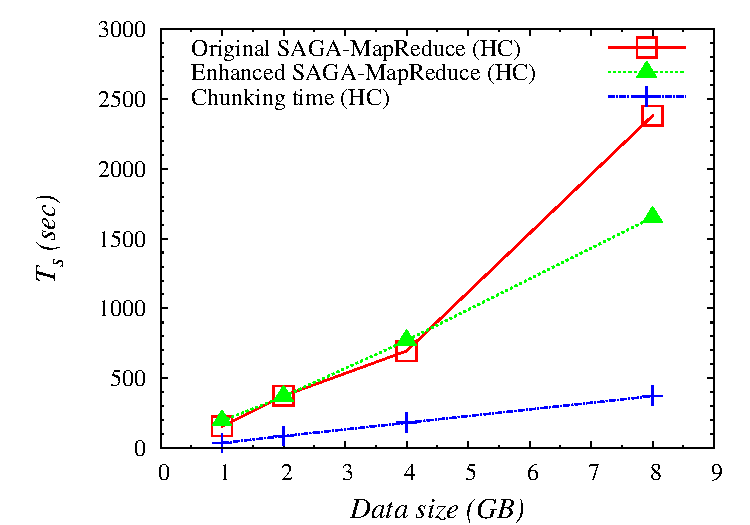
\includegraphics[width=0.5\textwidth]{figures/sagamr_comparison.pdf}
 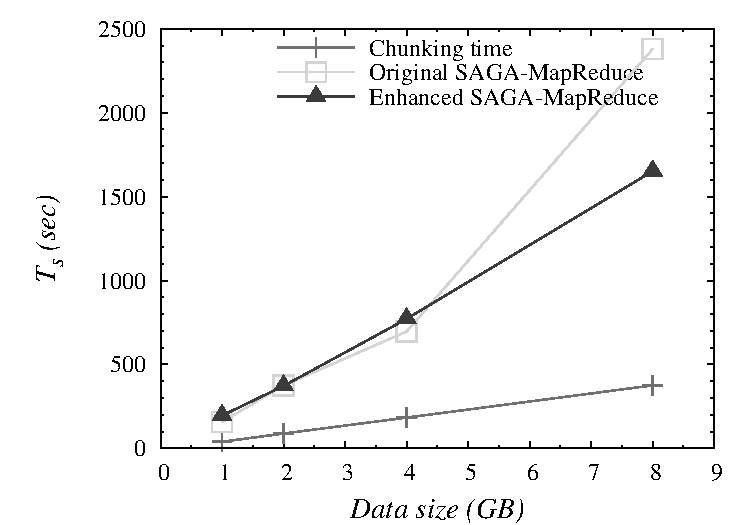
\includegraphics[width=0.8\textwidth]{figures/sagamr_comparison-gray.pdf}
 \caption{
   Comparison of enhanced SAGA-MR performance versus
   early-version of SAGA-MR on the ILAB cluster using 8 workers running on 8
   physical machines. Jobs were launched via SSH and used NFS for file
   operations.
   \label{fig:sagamr_comparison}
   }
   \alnote{do we have a scalable version of this picture}
\end{figure}

\subsection{Type II ALI: Application Performance Using SAGA-based
Sphere and MapReduce}

\subsubsection{Experiment I -- Varying chunk sizes} 

For the Sector-Sphere based \wc, Sector maintains and tracks data in
the cloud at the file level. There is no support in Sphere to control
the chunk sizes of files assigned to the Sphere processing
engines. Therefore, to experiment with different chunk sizes, the
files were split manually into smaller chunks before the \wc
application was launched. In this set of experiments, we vary the
chunk size from 16 MB to 256 MB, while keeping the number of SPEs
constant at 8, and the data size constant at 4 GB. Each SPE is running
on a separate physical node in the cluster. These results are
presented in Fig.~\ref{fig:sphere_mr_chunksize}.  Note that both data
and computation were distributed for these experiments.  As evident
from the results we collected, a correlation exists between the chunk
sizes and performance of Sphere.  As the chunk sizes increase, the
performance deteriorates. In particular, we observe a decline in
performance after the 64 MB data, in that there is an increase in the
gradient of the plot, after chunk sizes have reached 64 MB.

% \jhanote{Please describe the configurations used for Sphere and
%   MapReduce explicitly (distributed-distributed?).}
%\jhanote{With the new data, does this
%  still hold? ie., 64 MB or do we remove this sentence?}

\begin{figure}[htb!]
 \dnnn\dnnn
 \centering
 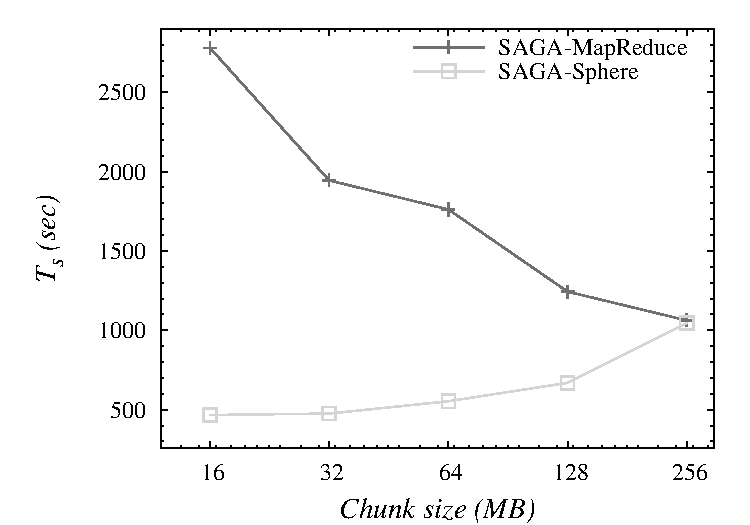
\includegraphics[width=0.8\textwidth]{figures/sphere_mr_varying_chunksize-gray.pdf}
 \caption{
   Performance of \sagamapreduce (left axis) and
   SAGA-Sphere (right axis) when varying chunk size while keeping the amount
   of processed data constant at 4GBs. Data and computation were
   distributed for these experiments.
   \label{fig:sphere_mr_chunksize}
   }
\end{figure}

We performed the same set of experiments with SAGA-MapReduce based \wc
and observe a completely different performance trend as the chunk size
varied.  We use an HDFS file system running datanodes on each of the 8
workers and set the number of reduce tasks to 8.  In case of
SAGA-MapReduce, performance increases with larger chunk sizes,
reaching Sphere's performance at the 256 MB data point.  According to
our analysis, this can be attributed to the fact that for
SAGA-MapReduce, $t_{coord}$ can dominate the total time-to-solution
for large number of workers (or equivalently smaller chunk sizes).
The larger the chunk size, the smaller the number of map tasks
launched (workers), and provided the data work-load assigned to each
worker is not too high, $t_{coord}$ decreases with increasing chunk
size.


\subsubsection{Experiment II -- Varying Workers}

We perform two sets of experiments with SAGA-Sphere running the same
\wc application.  We keep the chunk size constant at 64 MB, the data
size fixed at 4GB (as previously) but vary the number of workers in
two configurations. In the first configuration, we use Sphere on a
local data and local compute configuration. In the second
configuration, we observe how the solution scales to a distributed
data and distributed compute configuration. These results are
illustrated in Fig.~\ref{fig:sphere_varying_workers}.  

\begin{figure}[htb!]
 \centering
 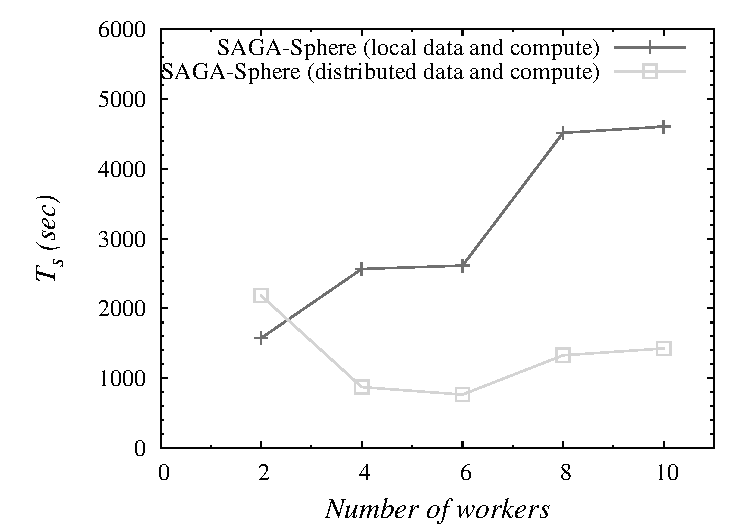
\includegraphics[width=0.8\textwidth]{figures/sphere_varying_workers-gray.pdf}
 \caption{
   Comparison of SAGA-Sphere performance when varying the number of workers
   between 2 and 10 in two configurations: (1) local data and computation
   and (2) distributed data and computation.
   \label{fig:sphere_varying_workers}
   }
\end{figure}

For the
local-local configuration, we launch Sector and Sphere on a single
physical node.  For the distribute-distribute configuration, we launch
Sector and Sphere on one physical node per SPE.  For the data-set
sizes considered, we observe good performance from 4 to 6 distributed
workers, before which the coordination costs due to the number of SPEs
starts to get high, with a concomitant increase in
time-to-solution. This is a nice but simple demonstration of the
advantage of distribution (logically distributed in this case, if not
physically distributed). Sector can maintain file replicas to achieve
optimal data distribution between SPEs and minimize synchronization
overhead. For the purpose of our experiments, we limited Sector to not
create any replicas.

\begin{figure}[htb!]
 \dnnn\dnnn
 \centering
 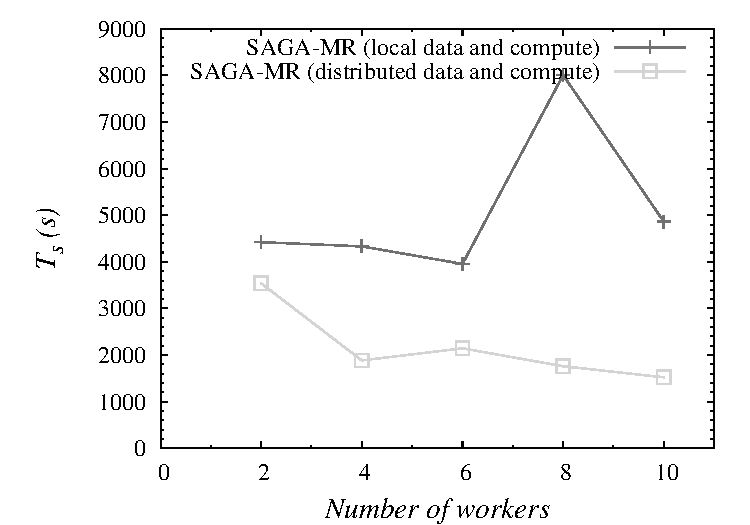
\includegraphics[width=0.8\textwidth]{figures/sagamr_varying_workers-gray.pdf}
 \caption{
   Comparison of \sagamapreduce when varying the number of workers
   between 2 and 10 in two configurations: (1) local data and computation
   and (2) distributed data and computation.
   \label{fig:sagamr_varying_workers}
   }
\end{figure}
% \miklosnote{Shantenu: Please correct figure placement as needed.}
% \jhanote{this is ok, i think}

We perform similar measurements via \sagamapreduce: while keeping the
chunk size constant at 64MB and the data size at 4GB, we note the
time-to-solution of the \wc application in the two configurations
described for SAGA-Sphere above.  For the distribute-distribute
configuration we use HDFS as the distributed file system and launch
jobs using the SAGA SSH job adaptor.  In contrast to the varying chunk
size experiments, we set the number of reduce tasks to be equal to the
number of workers spawned.  \jhanote{I can't determine where we
  establish that for varying chunk size we say that the number of
  workers in the map phase is not the same as the reduce phase. We
  only say that the number of reduce workers is set to 8 and imply
  that it is kept fixed.} For the local-local configuration we launch
workers on the machine running the master as separate processes and
use the local file system for file operations.  As can be seen in
Fig.~\ref{fig:sagamr_varying_workers} \sagamapreduce scales as
expected in the distribute-distribute configuration.  However, for the
local-local configuration performance degrades when adding more
workers.  Since each map task writes as many files as the number of
reduce tasks at the same time, and each reduce task needs to read from
as many files as the number of input chunks, the number of concurrent
disk I/O increases very quickly\jhanote{Miklos, please check, I did
not change the meaning of what was intended}; this can cause a
bottleneck when performing computations on one physical node (I/O
system).  According to Fig.~\ref{fig:sagamr_varying_workers} the
optimal number of workers is 6 for the local-local configuration.  We
did not include results for more than 10 workers in order to preserve
the linear
scale. % \miklosnote{Shall we note why we don't include results for 10
%   workers in the local-local configuration (takes toooooo much
%   time)?}\jhanote{done}

SAGA gives us the opportunity to experiment with different programming
models very easily.  As evident from the data plots in
Fig.~\ref{fig:sphere_mr_chunksize}, certain behavioral trends for
SAGA-Sphere and \sagamapreduce emerge.  In Experiment 1, where we keep
the number of workers constant and vary the chunk sizes, the trends
between \sagamapreduce and Sphere are inversed: the Sphere performance
deteriorates with increasing chunk sizes, while the performance of
\sagamapreduce increases. This behavior suggests that \sagamapreduce's
synchronization overhead to manage smaller chunk sizes compared to the
speed up achieved through parallelism is much higher.  In the case of
the \wc application, \sagamapreduce appears to be more suitable for
coarse grained computations. SAGA-Sphere, on the other hand, yields
better performance from smaller chunks sizes (a larger amount of
files) making it suitable for finer grained computations with better
data distribution.

In Experiment 2, where we keep the chunk size to a constant of 64 MB,
SAGA-Sphere exhibits a trend where adding more SPEs has a positive
impact on performance. However, at the 8 SPEs and 10 SPEs data points,
we see a decline in performance, possibly due to high synchronization
costs between the workers. What is interesting to notice are the two
data points at 64 MB chunk size and at 16 MB chunk size for
SAGA-Sphere in Fig.~\ref{fig:sphere_mr_chunksize}.  Reducing the chunk
size by 75\%, thereby providing better data distribution with a larger
number of files, we see almost a 65\% increase in performance. This
further confirms our supposition that good data distribution had a
major impact on Sphere's performance for the \wc application. We do
not claim that fine grained computation granularity is a concrete
determinant of SAGA-Sphere's performance in a general case, but a
noticeable aspect that emerges through its comparison with
\sagamapreduce.


\subsection{Type III ALI: Interoperability Concurrency}

We discuss the third type of interoperability in this section,
where SAGA-MapReduce and SAGA-Sphere are used in conjunction 
to solve the \wc problem. We first use the 'netperf' 
utility to measure the throughput from the client host to 
the \sagamapreduce master node and SAGA-Sphere master node. 
In our case, the throughput measured to the two nodes was 
approximately equal (935 MB/s to SAGA-Sphere and 925 MB/s to SAGA-MapReduce). 
Based on these metrics, we split the 4.0 GB data set 
into two equal 2.0 GB parts. This is to ensure that the data 
transfer time to both masters is approximately the same. We 
configured both systems to utilize 4 workers each 
and 64 MB chunk sizes. The data transfer time to the Sector 
cloud took a total of 97.8 seconds and 10.4 seconds to the 
SAGA-MapReduce master node. The longer transfer time to Sector 
can be credited to the overhead incurred from registering 
the files in Sector. The data transfer was done sequentially. 
\miklosnote{Should describe here the configurations used for Sphere and
MapReduce too.}

We found that SAGA-Sphere took a total of 441.3 seconds to process the
2.0 GB data, while \sagamapreduce took a total of 769
seconds. Aggregating the output results from the two systems took a
negligible amount of time (only 0.9 seconds). The data was already
sorted and hence could be merged in almost constant
time. % O(n) complexity.
The above simple experiment of combining two varied programming models
for solving a common problem paves the way to further investigation
into smarter data and compute placement techniques.  The total time
taken to execute the \wc application in this case was approximately
877.9 seconds. It is interesting to note that this performance measure
lies between 1329.96 seconds for 8 SPEs and 716 seconds for 8
SAGA-MapReduce workers at a 64 MB chunk size.

\section{Interoperability Experiments: Ensemble of Biomolecular
  Simulations}

Several classes of applications are well suited for distributed
environments. Probably the best known and most powerful examples are
those that involve an ensemble of decoupled tasks, such as simple
parameter sweep applications~\cite{1239909}. In the following
we investigate an ensemble of (parallel HPC) MD simulations. 
Ensemble based approaches represent an important and promising attempt
to overcome the general limitations of insufficient time-scales, as
well as specific limitations of inadequate conformational sampling
arising from kinetic trappings.  The fact that one single long-running
simulation can be substituted for an ensemble of simulations, make
these ideal candidates for distributed environments.  This 
provides an important general motivation for researching ways to
support scale-out and thus enhance sampling and to thereby increase
``effective'' time-scales studied.

The physical system we investigate is the HCV internal ribosome entry 
site and is recognized specifically by the small ribosomal subunit and 
eukaryotic initiation factor 3 (eIF3) before viral translation initiation.  
This makes it a good candidate for new drugs targeting HCV. 
The initial conformation of the RNA is taken from the NMR
structure (PDB ID: 1PK7).  By using multiple replicas, the aim is to
enhance the sampling of the conformational flexibility of the molecule
as well as the equilibrium energetics. NAMD~\cite{Phillips:2005gd} is
used as MD code.

To efficiently execute the ensemble of batch jobs without the necessity to queue 
each individual job, the application utilizes the SAGA BigJob 
framework~\cite{saga_bigjob_condor_cloud}. BigJob is a  
Pilot-Job framework that provides the user a uniform abstraction to grids and clouds
independent of any particular cloud or grid provider that can be
instantiated dynamically. Pilot-Jobs are an execution abstraction that have 
been used by many communities to increase the predictability and time-to-solution of
such applications.  Pilot-Jobs have been used to (i) improve the
utilization of resources, (ii) to reduce the net wait time of a
collection of tasks, (iii) facilitate bulk or high-throughput
simulations where multiple jobs need to be submitted which would
otherwise saturate the queuing system, and (iv) as a basis to
implement application specific scheduling decisions and policy
decisions.

As shown in Figure~\ref{fig:figures_distributed_pilot_job}, BigJob currently
provides an abstraction to grids, Condor pools and
clouds. Using the same API, applications can dynamically allocate
resources via the big-job interface and bind sub-jobs to these
resources. 

\begin{figure}[htbp]
    \centering
    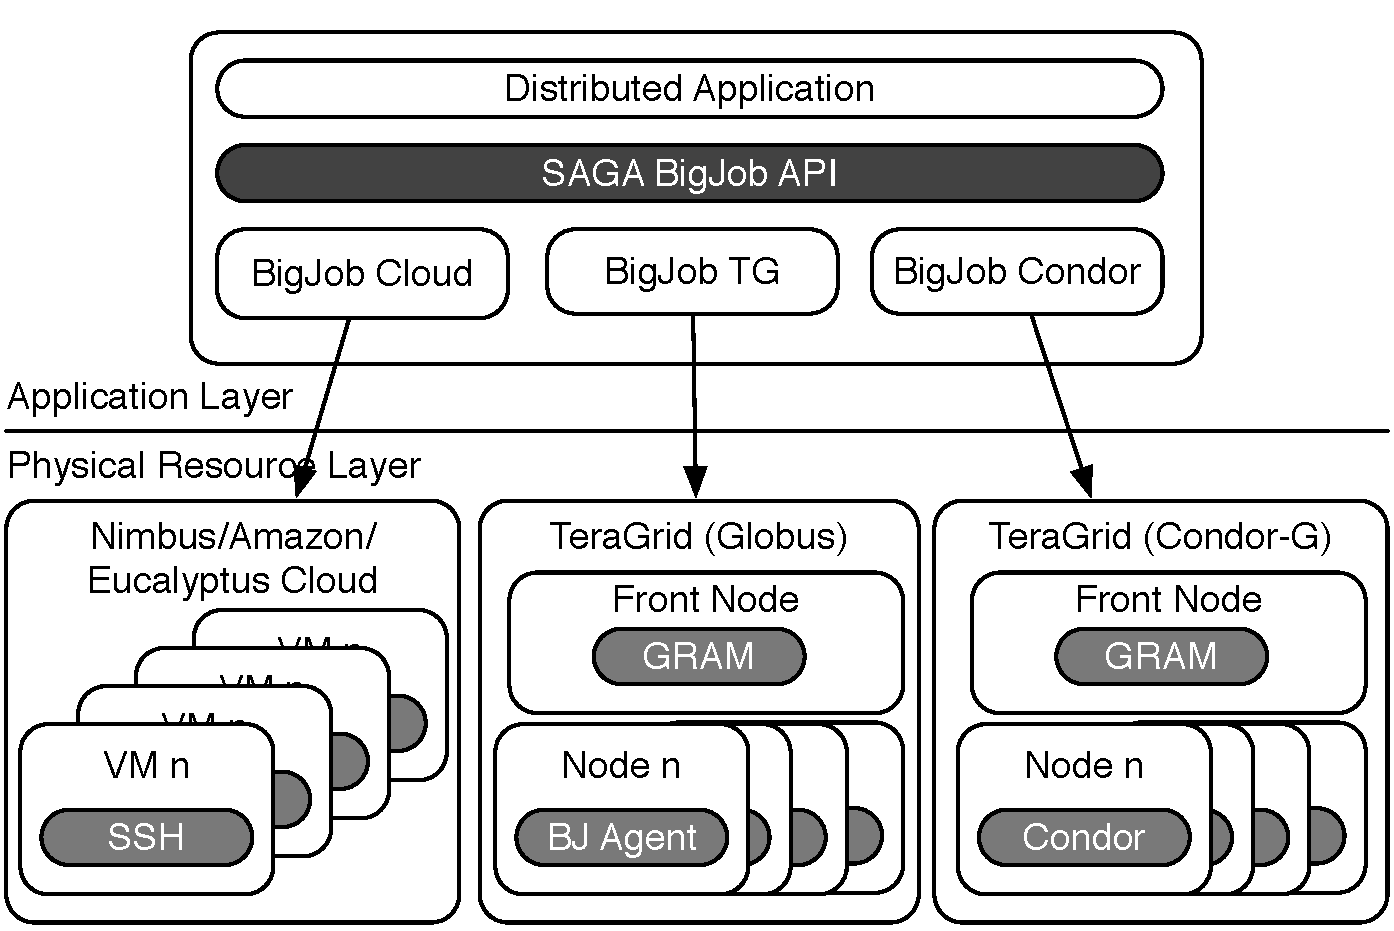
\includegraphics[width=0.9\textwidth]{figures/distributed_pilot_job.pdf}
    \caption{
      \footnotesize
      \label{fig:figures_distributed_pilot_job}
      An overview of the SAGA-based Pilot Job:     The SAGA Pilot Job API 
      is currently implemented by three different backends - one for grids,
      Condor and for clouds.}
\end{figure}

In the following we use an ensemble of MD simulations to investigate different 
BigJob usage modes and analyze the time-to-completion \tc in different scenarios.


\subsection{Scenario A: \tc for Workload for Different Resource
  Configurations\\}

\alnote{Not sure whether we should introduce ensemble-based approaches
  as programming models for type II and III interop?? Probably too
  artificial.} \jhanote{I agree that it would be too artificial. I
  have put a note about Type I interop}

In this scenario and as proof of scale-out capabilities using type I
interoperability provided by SAGA, we use SAGA-BigJob (a higher-level
package) to run replicas across different types of infrastructures
%(type I interoperability).
% , the LONI clusters -- Poseidon, Oliver, and the Nimbus Cloud.
At the beginning of the experiment a particular set of Pilot-Jobs is
started in each environment. Once a Pilot-Job becomes active, the
application assigns replicas to this job.  We measure \tc for different
resource configurations using a workload of 8 replicas each running on
8 cores. The following setups have been used
\begin{itemize}
\item Scenario 1 (A1): Resource I and III -- Clouds and GT2 based grids. 
\item Scenario 2 (A2): Resource II and III -- Clouds and Condor grids.
\item Scenario 3 (A3): Resource I, II and III -- Clouds, GT2 and Condor grids.
\end{itemize} 
For this experiment the LONI clusters: Poseidon and Oliver are used as
grid and Condor resources and Nimbus as cloud resource.

\begin{figure}[tbp]
    \centering
        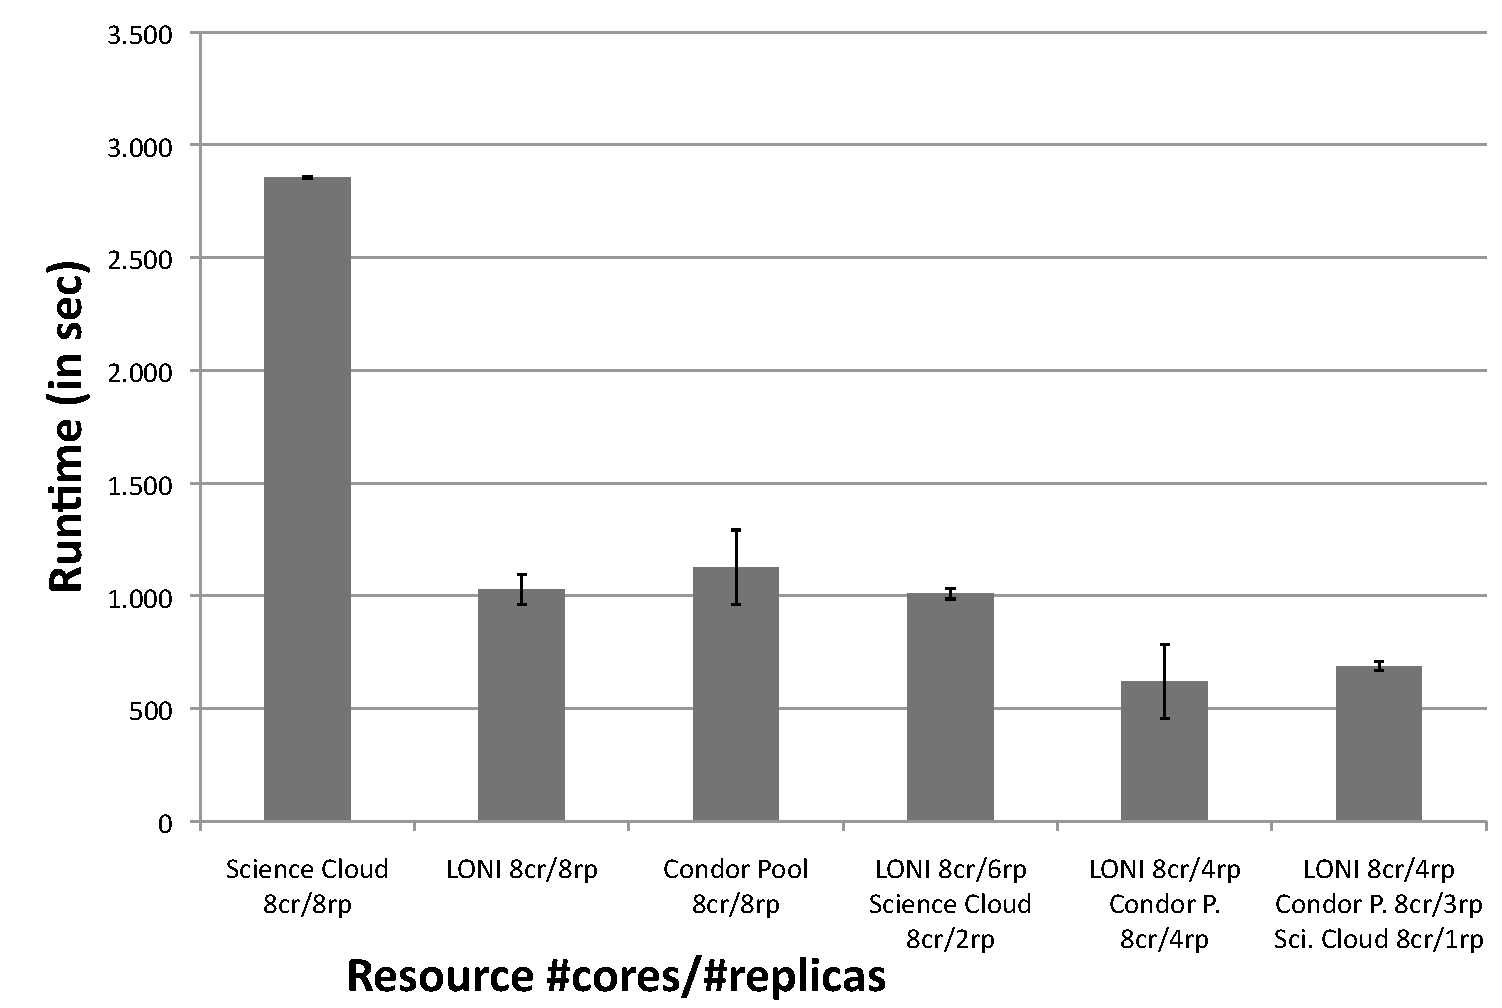
\includegraphics[width=0.8\textwidth]{figures/8replica_scenario_grid_condor_cloud}
        \caption{
          \footnotesize
          \label{fig:performance_8replica_grid_cloud_condor}
          \textbf{A1 - A3: Collective Usage of Grid, Condor and
          Cloud Resources for Workload of 8 Replicas: } The experiments showed 
          that if the grid and Condor resource Poseidon has only a light load, 
          no benefits for using additional cloud resources exist. However, the 
          introduction of an additional Condor or grid resource significantly 
          decreases \tc.}
\end{figure}

Figure~\ref{fig:performance_8replica_grid_cloud_condor} shows the
results. For the first three bars, only one infrastructure was used to
complete the 8-replica workload. Running the whole scenario in the
Science Cloud resulted in a quite poor but predictable performance --
the standard deviation for this scenario is very low. The LONI
resources are about 3 times faster than the Science Cloud, which
corresponds to our earlier findings.  The performance of the Condor
and grid BigJob is similar, which can be expected since the underlying
physical LONI resources are the same.  Solely, a slightly higher
startup overhead can be observed in the Condor runtimes.

In the next set of 3 experiments, multiple resources were used. For
Scenario A1 (the fourth bar from left), 2 replicas were executed on
the Science Cloud. The offloading of 2 replicas to an additional cloud
resource resulted in a light improvement of \tc compared to using
just LONI resources. Thus, the usage of cloud resources must be carefully
considered since \tc is determined by the slowest resource, i.e., Nimbus. As
described earlier, the startup time for Nimbus images is in particular
for such short runs significant. Also, NAMD performs significantly
worse in the Nimbus cloud than on Poseidon or Oliver. Since the
startup time on Nimbus averages to 357\,sec and each 8 core replica runs
for about 363\,sec at least 720\,sec must be allowed for running a single replica on
Nimbus. Thus, it can be concluded that if resources in the grids or
Condor pool are instantly available, it is not reasonable to start
additional cloud resources.  However, it must be noted that there are
virtual machines types with a better performance available, e.g., in
the Amazon cloud. These VMs are usually associated with higher costs
(up to 2.40\,\$ per CPU hour) than the Science Cloud VMs. For a
further discussion of cost trade-offs for scientific computations in
clouds see Deelman et\,al.~\cite{1413421}.


\subsection{Scenario B: Investigating Workload Distribution 
            for a Given $T_{max}$\\}

Given that clouds provide the illusion of infinite capacity, or at
least queue wait-times are non-existent, it is likely that when using
multiple resource types and with loaded grids/clusters (e.g., TeraGrid
is currently over-subscribed and typical queue wait times often exceed
24hours), most sub-jobs will end up on the cloud infrastructure.
Thus, in Scenario B, the resource assignment algorithm we use is as
follows: We submit tasks to non-cloud resources first and periodically
monitor the progress of the tasks. If insufficient jobs have finished
when time equal to $T_{X}$ has elapsed (determined per criteria
outlined below),
%(completion being  reached at current rates of progress),
%(defined as: \tmax - 2 average \tc on all Clouds)  
than we move the workload to utilize clouds.  The underlying basis is
that clouds have an explicit cost associated with them and if jobs can
be completed on the TG/Condor-pool while preserving the performance
constraints, we opt for such a solution. However, if queue loads
prevent the performance requirements being met, we move the jobs to a
cloud-resource, which we have shown has less fluctuation in \tc of the
workload.

For this experiment we integrated a progress manager that implements
the described algorithm into the replica application.  The user has
the possibility to specify a maximum runtime and a check interval.  At
the beginning of each check interval the progress manager compares the
number of jobs done with the total number of jobs and estimates the
total number of jobs that can be completed within the requested
timeframe. If the total number of jobs is higher than this estimate,
the progress monitor instantiates another BigJob object request
additional cloud resources for a single replica.  In this scenario,
each time an intermediate target is not met four additional Nimbus VMs
sufficient for running another eight core replica are instantiated.

%Table~\ref{tab:app_deadline} summarizes the results.
% \begin{table}
% %	\begin{tabular}{|l|l|l|}
% 	\hline
%     Result & \#\,Occurrences &Average \tc \\ \hline
% 	No VM started &6 &7.8\,min\\ \hline
% 	1 VMs started &1 &36.4\,min\\ \hline
% 	2 VMs started &1 &47.3\,min\\ \hline
% 	3 VMs started &2 &44.2\,min\\ \hline
% %	\end{tabular}
% 	\caption{\footnotesize  Usage of Cloud Pilot-Jobs to Ensure Deadline \label{tab:app_deadline}}
% \end{table}

% \begin{table}[ht]
%     \centering
% 	\begin{tabular}{|l|l|l|}
% 	\hline
%     Result & \#\,Occurrences &Average \tc \\ \hline
% 	No VM started &6 &7.8\,min\\ \hline
% 	1 VMs started &1 &36.4\,min\\ \hline
% 	2 VMs started &1 &47.3\,min\\ \hline
% 	3 VMs started &2 &44.2\,min\\ \hline
% 	\end{tabular}
% 	\caption{
%     \footnotesize
%     Usage of Cloud Pilot-Jobs to Ensure Deadline \label{tab:app_deadline}}
% \end{table}

In the investigated scenario, we configured a maximum runtime of
45\,minutes and a progress check interval of 4 minutes. We repeated
the same experiment 10\,times at different times of the day. In 6 out
of 10\,cases the scenario completed in about 8\,minutes. However, the
fluctuation in particular in the waiting time on typical grid
resources can be very high. Thus, in 4 cases it was necessary to start
additional VMs to meet the application deadline.  In two cases
3\,Pilot-Jobs each with 8 cores had to be started, and in one case a
single Pilot-Job was sufficient.  In a single case the deadline was
missed solely due to the fact that not enough cloud resources were
available, i.e., we are only able to start 2 instead of 3
Pilot-Jobs.

\section{Future Work: Windows Azure}

\jhanote{Azure section will need refinement} \alnote{Are we solely
  targeting Type I interoperability or do we aim for type II and III?}
\jhanote{Yes, we're using Type I here too ONLY I think, although there
  is scope for type II/III interop too, but we're not there yet.}

As alluded to in earlier parts of this chapter, we have investigated
and analyzed multiple platforms -- existing (GT2-based canonical
Grids) and emerging infrastructure (EC2). Azure is an emerging cloud
platform developed and operated by Microsoft.  Azure provides
different abstractions, building blocks for creating scalable and
reliable scientific applications without the need for on-premise
hardware; we believe Azure-based abstractions and services have the
potential to be very effective in the design, development and
deployment of distributed applications. Due to these capabilities, we
will focus on Azure in the closing section of this chapter, but as
many details are still being worked out, we present this analysis as
future (high-potential) work.

Azure follows the platform as a service paradigm offering an
integrated solution for managing compute and data-intensive tasks as
well as web applications. The platform is able to dynamically scale
applications without the need to manually manage tasks and deployments
on virtual machine level. After a brief introduction of the
abstractions that are provided of Azure, we discuss how Azure's
abstractions and capabilities can be utilized for ensemble-based
bio-molecular simulations of the type discussed in \S6.

\subsection{Understanding Azure-system Abstractions}

Azure provides different higher level services, e.\,g.\ the Azure
AppFabric or Azure Storage, that can be accessed via HTTP/REST from
anywhere. Windows Azure offers a platform for on-demand computing and
for hosting generic server-side applications. The so-called Azure
fabric controller automatically monitors alls VMs, automatically
reacts to hardware and software failures and manages application
upgrades.

\subsubsection{Compute}
Windows Azure formalizes different types of virtual machines into
so called roles. Web roles e.\,g.\ are used to host web applications
and frontend code, while worker roles are well suited for background
processing. While these roles target specific scenarios, they are also
highly customizable. Worker roles can e.\,g.\ run native code. The
application must solely implemented a defined entry point, which is
then called by Azure. The Azure fabric controller automatically
manages and monitors applications, handles hardware and software
failures as well as updates to the operating system or to the
application.  Commonly, scientific applications utilize worker roles
for compute- and data-intensive tasks. AzureBlast~\cite{azure_blast}
e.\,g.\ heavily relies on worker roles for computing bio-sequences.

\subsubsection{Storage}
For storing large amounts of data the Azure storage platform
provides three key services: the \emph{Azure Blob Storage} for storing
large objects of raw data, the \emph{Azure Table Storage} for
semi-structured data and the \emph{Azure Queue Storage} for
implementing message queues.  The data is storage replicated across
multiple data centers to protect it against hardware and software
failures. In contrast to other cloud offerings (e.\,g.\ Amazon S3) the
Azure Storage Services provide strong consistency guarantees, i.\,e.\
all changes are immediately visible to all future calls. While
eventual consistency as implemented by S3~\cite{1294281} usually
offers a better performance and scalability, it has some disadvantages
mainly caused by the fact that the complexity is moved to the
application space.

The blob storage can store file up to a size of 1\,TB, which makes it
particularly well suited for data-intensive application. The Amazon S3
service e.\,g.\ restricts the maximum file size to 5\,GB. Further, the
access to the blob storage can be optimized for certain usage modes:
\emph{block blob} can be split into chunks which can be uploaded and
downloaded separately and in parallel.  Thus, block blobs are well
suited for uploading and streaming large amounts of data. \emph{Page
  blob} manage the storage as an array of pages. Each of these pages
can be addressed individually, which makes page blobs a good tool for
random read/write scenarios. \emph{Azure XDrive} provides a durable
NTFS volume, which is backed by a page blob. In particular legacy
applications that heavily utilize file-based storage can simply be
ported to Azure using XDrive.

The Azure Queue Service provides a reliable storage for the delivery
of messages within distributed applications.  The queue service is
ideal to orchestrate the various components of a distributed
applications, e.\,g.\ by distributing work packages or collecting
results, which could be running on Azure or on another resource,
e.\,g.\ a science cloud.

The Azure Table Storage is ideally suited for storing structured
data. Unlike traditional relational database systems, the table
storage is designed with respect to scale-out, low cost and high
performance similar to Google's BigTable~\cite{bigtable2006}
system. For legacy application Azure also provides a SQL-Server based,
relational datastores called SQL Azure. In contrast to Azure tables,
SQL storage supports common relation database features, such as
foreign keys, joins and SQL as query language.


\subsection{Azure: Understanding the Applications}

The Azure platform provides many capabilities and characteristics that
are useful for scientific applications. Clouds like Azure are
particularly well suited for loosely-coupled applications that demand
a large number of processors, but do not require a low latency
interconnect. 

% Table~\ref{tab:app_azure_mapping} maps the requirements
% of the scientific applications in \S2 to the abstractions/services of
% the Azure platform.
% \begin{table}[t]
%     \centering
%     \footnotesize
%     \hspace*{-1em}
%     \begin{tabular}{|p{3cm}|p{6cm}|p{6cm}|}
%           \hline
%           \textbf{Application} &\textbf{Necessary Azure Services} &\textbf{Additional Capabilities}\\
%           \hline
%           \multirow{2}{3cm}{\textbf{Bio-EnMD}}
%           &\bull Blob/Queue/Table Storage  &\bull  Pilot-Jobs \\
%           &\bull Worker/Web Roles &\bull Adaptive/Autonomic Scheduling\\
%           &                       &\bull MPI-Support \\
%           \hline
%           \multirow{2}{3cm}{\textbf{EnKF-Based Sequestration}}
%           &\bull Blob/Queue/Table Storage  & \bull Pilot-Jobs\\
%           &\bull xDrive                     & \bull Data management system\\
%           & \bull Worker/Web Roles           & \bull Adaptive/Autonomic Scheduling\\
%           \hline
%           \multirow{2}{3cm}{\textbf{DAG-based Montage}}  
%           &\bull Blob/Queue/Table Storage     
%           &\multirow{2}{5.6cm}{\bull Workflow engine with support for dynamic 
%             and distributed workflows (modeling and enactment)}        \\
%           &\bull Worker/Web Roles             & \\
%           &\bull AppFabric (Service Bus)      &\\
%           \hline
%           \multirow{2}{3cm}{\textbf{MapReduce-based Genome App.}}
%           &\bull Blob/Queue/Table Storage       &\bull Dryad\\         
%           &\bull Worker/Web Roles               &\bull Distributed filesystem\\             
%           \hline
%     \end{tabular}
%     \upp
%     \caption{Scientific Applications and Windows Azure}
%     \upp\upp
%     \label{tab:app_azure_mapping}
% \end{table}
Although loosely-coupled ensemble-based simulations are
computationally well suited for cloud infrastructures, coordinating
multiple ensemble-members remains a challenge, as does
data-management.
% A growing limitation in all these
% scenarios is that workflow, data management, and analysis have become
% rate limiting steps. 
In the following we discuss a generic Azure-based architecture that
addresses these concerns and is able to facilitate a range of
applications execution scenarios.

\subsubsection{Azure and Bio-EnMD}
\begin{figure}%{R}{0.4\textwidth}
    \centering
   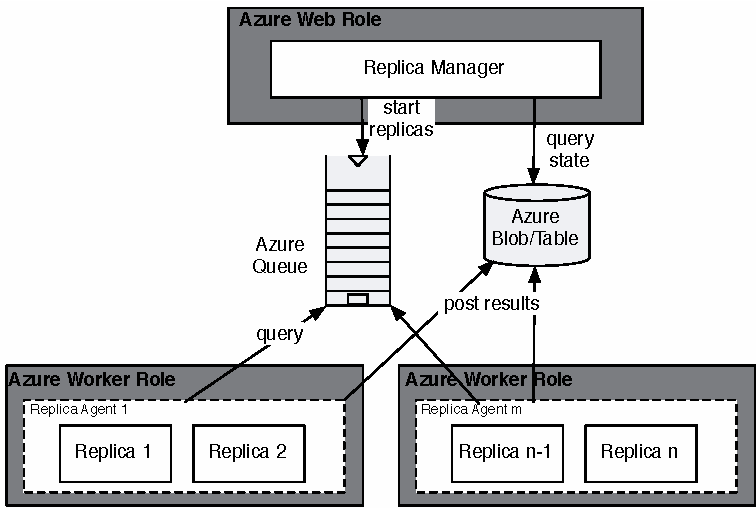
\includegraphics[width=0.8\textwidth]{figures/re-azure-gray}
    \caption{\textbf{Azure-based Bio-Ensembles:} The ensemble-based
      application utilizes the queue storage for distributing work
      packages from the Replica Manager running on a web role to the
      replica agents running on multiple worker roles.}
    \label{fig:figures_re_azure}
\end{figure}
Figure~\ref{fig:figures_re_azure} illustrates an example of a
framework for ensemble-based simulations built on top of the Azure
building blocks. The Replica Manager (RM), also called Ensemble
Manager, utilizes a web role to communicate with the end-user. This
role is mainly responsible for accepting simulation requests from the
end-user and for orchestrating the simulation runs. Later these
capabilities can be extended by supporting more advanced steering and
visualization features. The RM creates work packages -- the so called
\emph{replicas}, distributes them via the Azure Queue Service and
later collects the results stored by the replicas in the Azure
storage.  The Replica Agents run within Azure worker roles, which are
ideally suited for running background tasks. Azure enables users to
run native code within worker roles, i.\,e.\ the framework will be
able to support numerous MD codes, e.\,g.\ NAMD~\cite{Phillips:2005gd}
and AMBER~\cite{cheatham-5}.  Azure currently does not support MPI
computations across multiple worker roles, thus each MD
simulation is limited to 8 cores.

The worker roles running the replica agent are managed by the RM using
the Azure Service Management API. In the initial version we will
support the automatic start and stop of hosted services. In the final
version there will be a possibility to automatically deploy agent code
without the need to pre-configuring the VMs. Once the agents are
started, they query the Azure queue for new work items. If a work item
is found, a simulation task is started, e.\,g.\ by running the requested
MD code with right parameters.  The number of
MD jobs per worker role depends on the size of the worker role --
Azure currently supports worker roles up to 8 cores.

% \alnote{Kalman Filter option: we need to convey how we make decisions?
% we need to understand the various trade-offs}

The ensemble use case can greatly benefit from the
capabilities of Azure. If greater accuracy is required or a deadline
must be met, it can seamlessly scale-out to more worker roles.  The
Azure fabric controller monitors all VMs running the worker roles and
automatically restarts the worker roles if necessary. Further, Azure
provides various kinds of reliable and scalable storage options to
express different coordination schemes, e.\,g.\ the master-worker
communication can be conducted via the described message queue. 

\subsubsection{Azure and MapReduce}

For data-intensive applications, such as MapReduce-based applications,
Azure provides various interesting services: 
The blob storage is well suited for storing large amounts of file data, 
which can also be accessed via a NTFS file system. Data can be processed 
via worker roles. Further, Azure offers the possibility to express data/compute 
co-locations using so called affinity groups. MapReduce application require capabilities 
similar to the Bio-EnMD: mapping and reduction tasks can be spawned dynamically using the Service 
Management API. For storing and transferring data Azure provides various options
(xDrive versus block blob versus page blob). We will further evaluate these alternatives
in particular in comparison to distributed filesystems in the future. 


% \subsection{Assessment of Windows Azure}
% \upp
\subsection{Assessing Azure-system Abstractions and Applications}
% \upp
\begin{figure}[ht]
 \centering
 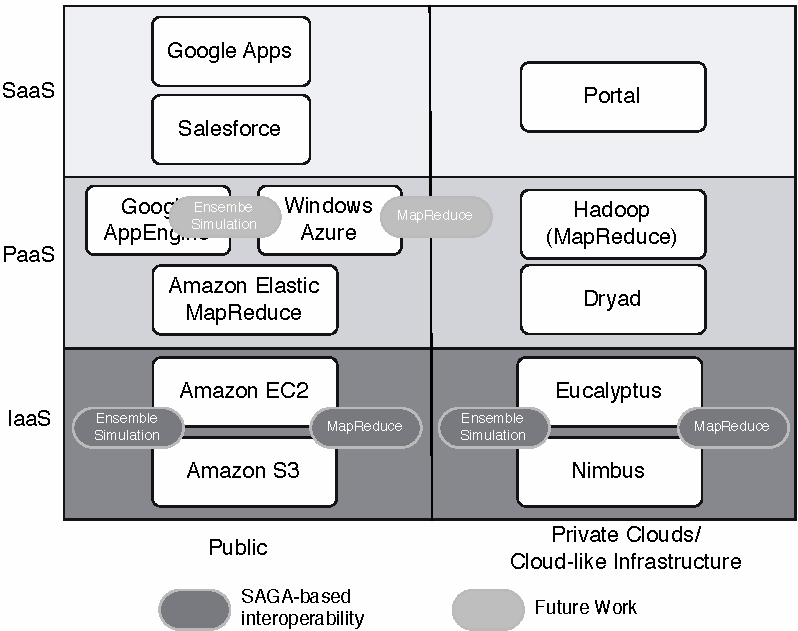
\includegraphics[width=0.8\textwidth]{figures/cloud_ontology_apps-gray}
 \caption{\footnotesize \textbf{Cloud Taxonomy and Application Examples}:
   Clouds provide services at different levels (IaaS, PaaS, SaaS).
   The amount of control available to users and developers decreases
   with the level of abstraction. According to their deployment model
   clouds can be categorized into public and private clouds.
   \label{fig:cloud_layers}}
   \upp\upp
\end{figure}

To aid an understanding of application characteristics suited to the
Azure platform, we briefly introduce a common categorization of cloud
services (see fig.~\ref{fig:cloud_layers}). The proposed service
layers consist of the following: the software as a service layer
(SaaS), the platform as a service (PaaS) layer and the infrastructure
as a service (IaaS) layer. Further, clouds can also be classified
according to their deployment model into public and private clouds
(for further details refer to~\cite{Jha:2010kx}).  Azure offers
services on the platform as a service layer and thus, generally
removes the need to manually manage low-level details as virtual
machine configurations, operating system installations and updates
etc.  At the same time worker roles provide an attractive environment
for running compute- and data-intensive applications. In contrast to
IaaS clouds, applications can benefit from features, such as failure
tolerance: the fabric controller e.\,g.\ monitors all applications
running in a role environment and restarts them if necessary.


Table~\ref{tab:saga-azure-mapping} illustrates how the
different Azure functionalities naturally map to existing SAGA API
packages, which covers job submission, file access and transfer, as
well as logical file management.  With very modest levels of effort,
applications will be able to utilize Azure in conjunction with many
other infrastructure types; also, a broad range of SAGA-based
application frameworks, such as Pilot-Jobs \& SAGA MapReduce 
will also become available and seamlessly
usable across multiple infrastructure as a consequence.


\begin{table}[ht]
\centering
  \footnotesize
  \begin{tabular} {cc}
    \hline
        \textbf{Azure Service} &\textbf{SAGA Package} \\ \hline
        Blob Storage &File API \\ \hline
        xDrive  &File API\\ \hline
        Table Storage &Advert API\\ \hline
        Service Management API &Job API\\ \hline
	\end{tabular}
	\caption{\textbf{SAGA-Azure Mapping:} This table illustrates how the different Azure services
	can be mapped to the different standardized SAGA API packages.} \label{tab:saga-azure-mapping}
\end{table}


% However, to efficiently enable science application
% to express such usage modes explicit application-level support is
% required.


% Several scientific applications from different domains (e.g., life
% sciences, high energy physics, astrophysics, computational chemistry)
% have been ported to cloud environments (see~\cite{Hill,Begin:2008rq,saga_grid_cloud_interop} 
% for examples). 

The majority of scientific applications (e.\,g.\ applications from life
sciences, high energy physics, astrophysics, computational chemistry)
that have been ported to cloud environments
(see~\cite{Hill,Begin:2008rq,saga_grid_cloud_interop} for examples),
rely on low-level IaaS cloud services and solely utilize static
execution modes: A scientist leases some virtual resources in order to
deploy their testing services. One may select different number of
instances to run their tests on. An instance of a VM is perceived as a
node or a processing unit. 
In contrast to traditional IaaS clouds, Azure provides different benefits: 
Azure operates on a higher level of abstractions and removes the need to manage details, such as
configuration and patching of the operating system. Azure applications
are declaratively described and packaged; the fabric controller
automatically handles the mapping of these applications to available
hardware.


% We engaged with Microsofts eXtreme Computing Group (Roger Barga) to assess
% Azure in a both theoretical and practical way. 

Azure provides several core services supporting various interesting
application characteristics and patterns. Com\-pute-intensive tasks can
naturally be mapped to worker roles, while the communication and
coordination between these roles is commonly done via the Azure
storage services. Worker roles can run not only run .NET code, but are
also capable of executing native code. However, Azure imposes some
limitations in the ability to scale up and out. The largest supported
VM has 8\,cores, 14\,GB of memory and 2\,TB of disk space.  Further,
MPI applications can currently not be run on Azure. While other IaaS
clouds can run MPI jobs, the performance usually degrades
significantly when running jobs across multiple VMs (see
figure~\ref{fig:performance_namd_run}a)). % \jhanote{Can first sentence
%   be merged into previous paragraph?}  While clouds support different
% application types, e.\,g. tightly and/or loosely-coupled applications,
% tightly coupled applications are less well suited, mainly due to the
% lack of high-end, low-latency interconnects.

% We have identified a representative set of physical problems
% applications that does

There exist a large number of physical problems that do not require
high-end HPC hardware and interconnects and can easily scale out on
Azure benefiting from the ability to acquire and release resources
on-demand.  An increasing number of applications directly target
distributed infrastructures instead of high-end machines. For example,
ensemble-based molecular dynamics approaches utilize multiple
sets of simulations of shorter duration instead of a single longer
simulation to support a more efficient phase-space sampling. Also,
such simulations often require the ability to acquire additional
resources, if e.\,g.\ a certain simulation event occurs that requires
the spawning of an additional replica.  Such an application can
greatly benefit from Azure capability to dynamically allocate
resources on demand. This capability is also useful for % EnKF-based
applications where the execution time and resource requirements cannot
be determined exactly in advance, either due to changes in runtime
requirements or interesting changes in application structure (e.\,g.\
different solver with different resource requirement or a different
workflow path~\cite{enkf_hybrid_grid_cloud}).


% There can be a multiple number of instances under the same VM, depending on
% the SLA one has agreed on. Once deploying the service, a scientist is
% ready to begin testing on the virtual nodes, likewise one would do on
% a traditional set of local clusters.

\begin{figure}[tbp]
  \centering
  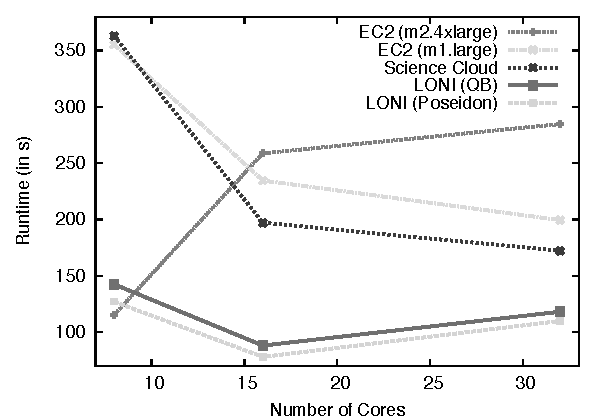
\includegraphics[width=0.45\textwidth]{figures/namd_run-gray.pdf}
  \label{tbd}
  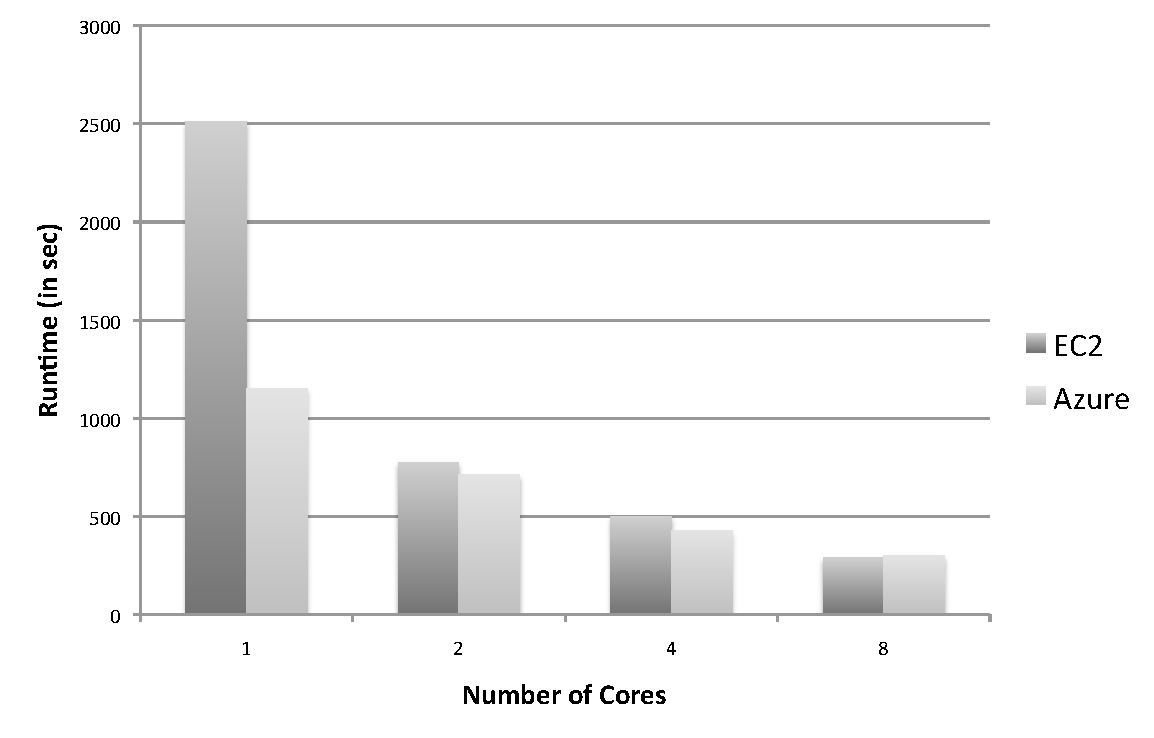
\includegraphics[width=0.5\textwidth]{figures/namd_ec2_azure}
  \label{fig:perf_namd_ec2_azure}
  \caption{\textbf{(a) NAMD Runtimes on Different Resource Types: }
    The graph shows that native HPC resource generally outperform
    cloud resources in particular when running applications across
    multiple nodes. However, the new high memory eight core EC2
    instance type was able to complete a replica run faster than QB or
    Poseidon. \textbf{(b) NAMD Performance on Azure and EC2:} In particular on
    smaller VM sizes Azure outperforms EC2.  On 8 core VMs EC2 shows a
    slightly better performance.}
   \label{fig:performance_namd_run}
\end{figure}

Most research has solely attempted to manually customize legacy
scientific applications in order to accommodate them into a cloud
infrastructure. Benchmark tests on both cloud infrastructures (EC2,
Azure) where a VM does not cross physical nodes, and conventional
computational clusters indicated no significant difference in the
performance as measured by execution (wall-clock) time and number of
processors used. Figure~\ref{fig:performance_namd_run}b presents an
initial performance assessment of Azure for MD simulations. Azure
outperforms
EC2; % Especially on smaller % instances Azure outperforms EC2. This
which is in noteworthy, since the costs for 2, 4 and 8 core VMs are
drastically lower on Azure. Since the underlying hardware is not known
one can only speculate about the reason. Microsoft controls the
hardware in its data center und optimizes its custom-built Azure
Hypervisor with respect to this hardware~\cite{Krishnan:2010nx}, which
could be a reason for the better performance. In summary, Azure offers
a good price/performance ratio in particular in comparison with EC2.


For data-intensive applications Azure provides several interesting
storage options: xDrive offers file system access to the Azure storage
service, which is in particular relevant for applications that manage
file-based data flows %, e.\,g.\ the EnKF application.
The blob storage is capable of storing large amounts of data -- a page
blob e.\,g.\ can store files up to a size of 1\,TB.  In comparison,
Amazon S3 is only capable of storing file with a size of up to 5\,GB,
the Google Storage for Developer file size limit is at 100\,GB. The
blob storage supports two different data access patterns: block blobs
are designed for continuous access, such as data streaming, while page
blobs can address each page individually and are particularly well
suited for random access. These properties can be mapped to the
characteristics of the respective application, e.\,g.\ a MapReduce
application usually accesses data in large chunks, which is well
supported by the block blob. In future we will investigate these
implementation alternatives and performance trade-offs in conjunction
with the proposed applications as part of this project.


\section{Discussion \& Conclusions}
\label{sec:discuss}

The aim of this chapter has been to show several types (and levels) of
interoperability; although driven by proof-of-capability experiments
and results therein, there are deeper questions that motivate this
work and define the research methodology.  As alluded to in the
opening section, the volume and the degree-of-distribution of data is
increasing rapidly; this imposes a need for applications to work
across a range of distributed infrastructures using several
programming models; this is consistent with the fact that it is not
possible to localize exa-bytes of data.  Thus, on the one hand there
is a need to decouple PM from infrastructures, and provide a range of
PM at the application developer's disposal. On the other hand, in
order to build empirical models, or validate existing predictions of
performance, it is important to establish \& experiment with
programming models and data-oriented algorithms (e.g., streaming) on a
range of systems. % This is an important step towards general-purpose
% programming models, the first-step of which is interoperability of the
% types discussed.
A critical and necessary step to achieve both is to provide
application-level interoperability as discussed.

In this chapter, we discussed two important (classes) of applications
-- data-intensive, \sagamapreduce \wc and compute-intensive
ensemble-based molecular-dynamics simulations. We posited three levels
of interoperability, and for \sagamapreduce \wc carried out
performance tests at all three levels. %  were performed using SAGA-\mr,
% which from an execution perspective is a relatively straight-forward
% application. 
At the lowest level, \sagamapreduce demonstrates how to
decouple the development of applications from the deployment details
of the run-time environment (Type I ALI).  It is critical to reiterate
that using this approach, applications remain insulated from any
underlying changes in the infrastructure -- not just grids and
different middleware layers, but also different systems with very
different semantics and characteristics, whilst being exposed to the
important distributed functionality.

With implementations of the two application frameworks -- SAGA based
Sector-Sphere and the \smr implementation, we also demonstrated Type
II ALI: applications can seamlessly switch between backends by
switching frameworks encapsulating different programming models.
Finally, by concurrently using Sector-Sphere \mr and \smr, we
demonstrated Type III ALI, allowing the application to span a wide
variety of backends concurrently, and efficiently.

Our approach does not confine us to \mr and applications based upon
\mr; SAGA is also capable of supporting additional programming models,
like Dryad.  We are also developing applications with non-trivial
data-access, transfer and scheduling characteristics \& requirements,
and deploying them on different underlying infrastructure guided by
heuristics to seek optimised performance.
% We will generalize our approach to most efficiently execute it by
% taking into consideration the data-locality, as well as the access
% patterns of the execution steps required to complete the work flow.
This analysis is done through developing performance models of
transferring data between frameworks, as well as the distribution of
the computing resources in the environment. Based on this analysis,
the data is placed efficiently, and a subset of nodes and frameworks
maybe chosen to perform the necessary computations. The shuffled data
is also cached for future computations.  We have embarked on the
creation of components that facilitate intelligence and flexibility in
data placement relative to the computational resource
~\cite{saga_dic_royalsoc09}. These components are connected in
frameworks using SAGA, thus further the agenda of general-purpose
programming models with efficient run-time support that can utilize
multiple heterogeneous resources.

In \S6, we showed how SAGA can be used to develop frameworks such as
infrastructure independent Pilot-Jobs, and demonstrated the
scaling-out over multiple distinct resources. Finally, in \S7 we
discussed Azure, some of the system-level abstractions that it
provides and analyzed how these can be utilized for ensemble-based
molecular dynamics simulations. We anticipate significant activity in
both scaling-up the use of Azure (for both applications discussed here
as well as other novel applications), as well as integrating Azure
with other infrastructure via the use of SAGA in the near future.


%\section{Acknowledgments}
\subsection*{Acknowledgments}

\small{ SJ acknowledges UK EPSRC grant number GR/D0766171/1 for
  supporting SAGA and the e-Science Institute, Edinburgh for the
  research theme, ``Distributed Programming Abstractions''.  SJ also
  acknowledges financial support from NSF-Cybertools and NIH-INBRE
  Grants, while ME acknowledges support from the grant OTKA NK 72845.
  We also acknowledge internal resources of the Center for Computation
  \& Technology (CCT) at LSU and computer resources provided by
  LONI/TeraGrid for QueenBee.  We thank Chris Miceli, Michael Miceli,
  Katerina Stamou, Hartmut Kaiser \& Lukasz Lacinski for their
  collaborative efforts on early parts of this work. We thank Mario
  Antonioletti and Neil Chue Hong for supporting this work through
  GSoC-2009 (OMII-UK Mentor Organization).}

\bibliographystyle{plain}
\bibliography{saga_data_intensive,cloud,saga}

\end{document}

% This work would not have been possible without the efforts and
% support of other members of the SAGA team.  In particular,
% \sagamapreduce was originally written by Chris and Michael Miceli,
% as part of a Google Summer of Code Project, with assistance from
% Hartmut Kaiser. We also thank Hartmut for great support during the
% testing and deployment phases of this project. We are greatful to
% Dmitrii Zagorodnov (UCSB) and Archit Kulshrestha (CyD group, CCT)
% for the support in deployment with Eucalyptus.  KS would like to
% acknowledge the LSU Networking Infrastructure \& Research IT
% Enablement team for their help and support.
